\documentclass[a4paper,12pt]{jreport}
\usepackage{amsmath}
% \usepackage[dvipdfmx]{graphics}
\usepackage[dvipdfmx]{graphicx}
%\documentstyle[a4j,12pt,epsf]{jreport}
\usepackage{url}
\usepackage{enumitem}
\usepackage{makecell}
\usepackage{subcaption}
\usepackage{tabularx}
\usepackage{array}
\usepackage{cite}


% margine control
\setlength{\textwidth}{16.5cm} \setlength{\textheight}{23.5cm}
\setlength{\oddsidemargin}{10pt} \setlength{\evensidemargin}{10pt}
\setlength{\topmargin}{-10pt} \setlength{\marginparsep}{15pt}
\setlength{\parskip}{0.3cm}

% reassignment of bib
\renewcommand{\bibname}{参考文献}


\title{{\Huge {\bf 卒業論文の書き方}}}

\author{{\LARGE {\bf 島川 博光}}}

\vspace{60mm}


\date{{\Large {\bf 2004年 12月}\\
              {\bf 2013年 1月 改訂}\\
              {\bf 2015年 8月 改訂}\\
              {\bf 2019年 2月 改訂}\\
              {\bf 2020年 1月 改訂}\\
              {\bf 2020年 9月 改訂}\\
              {\bf 2024年 12月 改訂}
	      }}


\begin{document}

\setlength{\baselineskip}{8mm}


\maketitle




\pagenumbering{roman}

\begin{center}
% {\LARGE {\bf 卒業論文の書き方}}


\vspace{10mm}

{\Large {\bf 概要}}
\end{center}

\addcontentsline{toc}{chapter}{概要}


\clearpage


\begin{center}
% {\LARGE {\bf How to Write Thesis}}


\vspace{10mm}

{\Large {\bf abstract}}
\end{center}

\addcontentsline{toc}{chapter}{abstract}

T

\clearpage


\addcontentsline{toc}{chapter}{目次}
\tableofcontents

\clearpage
\addcontentsline{toc}{chapter}{図目次}
\listoffigures
\clearpage
\addcontentsline{toc}{chapter}{表目次}
\listoftables

%%%%%%%%%%%%%%%%  End of Prologue   %%%%%%%%%%%%%%%%%%%%%%%%%%%%%%%%%%

\clearpage
\pagenumbering{arabic}

\chapter{はじめに}
現状の日本における少子高齢化に伴う生産年齢人口の減少は, 国内産業の持続性に関わる課題として指摘されている\bibitem{IPSS2023}. 特に工場などの作業現場を含む製造業では, 人手不足や技能継承, 生産性向上への対応が課題となりやすく, 省人化や現場データ活用（DX）の必要性が指摘されている\bibitem{METI2024Monozukuri,SMEA2024WhitePaper}. また, 生産工程等の現場職種において求人が需要超過となる状況も報告されている\bibitem{MHLWJobStats}.
一方で, 安全確保や進捗・品質の維持のためには, 限られた人員でも作業者の状態を継続的に把握する必要がある\bibitem{MHLWOSHMS}. これらを目視に依存して維持することには限界がある. 現場の状況把握には監視カメラが用いられることが多いが\bibitem{Yano2025CCTV}, 見通しが遮られる場合には対象を捉えられないという制約がある. また, 継続監視は注意の維持が難しく, 運用上は監視者の負荷が問題となり得る\bibitem{Donald2015,Dadashi2013}. さらに, 映像の自動解析を導入する場合も, 誤検出への対処やアラート設計等を含む運用設計が必要となる\bibitem{Dadashi2013}.

そこで近年, 視覚情報に依存しない手段として, ウェアラブルセンサにより身体動作の時系列データを取得し, そこから作業者の状態を推定する研究が進められている\bibitem{Bao2004}. 加速度などの慣性センサ時系列から行為を推定する手法や, 無線指標等を用いた屋内位置推定も広く研究されている\bibitem{Bahl2000,Youssef2005,Faragher2015}.
しかし, 現場の状態は時間, 場所, 行為に強く依存して変化する. 例えば「停止」は同一の行為として観測されるが, 荷下ろし地点付近での停止は作業の一部である一方, 通路中間での停止は滞留やトラブルの可能性を含む. また, 同じ地点にいても, 台車を押して通過しているのか荷下ろし作業を行っているのかで, 状況の解釈は異なる. よって, 行為推定や位置推定を単独で扱うだけでは, 作業者の状況把握に直結しにくい.

そこで本研究では, 状態をコンテキストとして扱い, コンテキストを「位置クラスと行為クラスの組」として定義する. この定義により, 推定結果を「どこで, 何をしているか」として解釈でき, 作業状態の把握や分析に接続しやすくなる.
位置と行為を統合して状況を推定する研究も報告されている\bibitem{Wang2024,Moreira2021}. ただし, 既存研究はセンサ構成, 環境条件, タスク設定などの前提に依存しやすく, 実環境へ適用する際には追加の調整や設計を要する場合が多い. また, 統合は位置と行為の同時正解を要するため, 個別の推定では不十分である. よって, 行為推定と位置推定を独立に設計し, 時刻同期により統合する枠組みが必要である.

本研究では, 行為と位置をそれぞれ独立かつリアルタイムに推定し, 推定結果を統合してコンテキストを判定し, 評価を行う手法を提案する. 提案手法では, 学習に用いる基準作業者と, 学習した推定モデルを適用する対象作業者を区別し, 役割を分割する. また, 既存の指標だけでは比較が不十分となる場合がある. そこで, 各推定に対して目的に合う評価指標を設計し, 実験で用いる.
行為の推定では, 教師情報の制約を軽減するため, 時系列クラスタリングにより状態列を生成し, これを擬似ラベルとして後段の学習に接続する. 位置の推定では, 受信指標の変動を前提として特徴量化と教師あり分類により位置クラスを推定する. 必要に応じて時間方向の整合を組み込むことで不自然な遷移を抑制する. 最後に, 行為推定結果と位置推定結果を同一時刻で統合し, 位置クラスと行為クラスの組としてコンテキストを判定する. 本手法は, 実環境における安全管理および作業内容把握の支援が期待できる.

本論文の構成は以下のとおりである. 2章では, コンテキスト推定に必要な構成要素や使用する手法について述べる. 3章では提案手法を示す. 4章では実験環境および取得データを示す. 5章から8章では各モデルの結果を示し, 影響する要因について考察する. 9章で本手法の限界を述べ, 10章で結論を述べる.


\chapter{関連研究}
\section{ウェアラブルHARと評価}
センサベースの行為認識（HAR）は, 加速度などの時系列信号を入力とし, 前処理, 特徴表現, 分類を経て行為クラスを出力する一連の処理として整理できる\bibitem{Bao2004}. HARの手法のうち, 特徴量抽出と古典的機械学習の組み合わせは実装容易性と計算量の点で優れている. 一方, 深層学習は表現学習により高精度化が進むが, データ分布や学習設定への依存が大きい\bibitem{Ordonez2016,Hammerla2016}. 特にエッジ実装では, 推論遅延や計算資源の制約が強く, 深層学習モデルは計算量の扱いが課題となる\bibitem{Zhou2025}.

また, 実環境では想定した性能が得られない場合がある. 実環境で性能が崩れる主要因は, 被験者の身体的条件の差およびウェアラブル端末の装着状態の差により, 学習時と推定時の分布が乖離する点にある\bibitem{Fallahzadeh2017,Banos2014Displacement}. このため, 汎化性とオンライン性を考慮した評価方法と設計が必要である. 評価では, 訓練データと評価データで被験者を分離し, 学習時と評価時で同一被験者が重複しないことを保証する. オンライン推定を想定する場合は推論遅延や計算資源を含めて報告する\bibitem{Zhou2025}.

本研究の行為推定は, エッジデバイスでのリアルタイム推定を想定し, 特徴量抽出と古典的機械学習に基づく軽量分類モデルで構成する.

\section{ラベル付与コスト削減}
教師ありHARでは, 遷移区間の曖昧さにより, ラベル付与に多くのコストを要する. このため, 大規模・継続的なデータ整備が難しいことが繰り返し指摘されている\bibitem{Saeed2019}. この問題の解決方法として, 無ラベルデータを活用するというものがある. 代表的な無ラベルデータの種類は2つあり, 自己教師あり学習による表現獲得をラベルにするものと, 疑似ラベルを介した自己学習の出力をラベルにするものがある\bibitem{Roy2024,Saeed2019}. HARで使用される自己教師あり学習は, センサからの出力を学習し, 下流タスクに適した形状に変換して出力する役割を担う. 近年は, 大規模な未ラベルデータを用いた自己教師あり学習により, 汎化性能を高める報告もある\bibitem{Yuan2024}. 一方, 完全教師なしで行為クラスそのものを安定に推定するのは依然難しいため, 実装上は表現学習や疑似ラベルを組み込んだ半教師ありの形で設計される例がある\bibitem{Roy2024,Saeed2019}.

以上を踏まえ, 本研究ではラベル付与コスト削減のために, 無ラベルの時系列データから疑似ラベルを生成し, これを教師情報として後段の学習に接続する. また, これらの手法は評価設定に依存しやすいため, 比較可能性を担保するには条件の明示が不可欠である\bibitem{Roy2024,Saeed2019}.

\section{時系列クラスタリング}
無ラベルの時系列データからラベル候補のセグメント系列を得る手法として, 時系列クラスタリングがある\bibitem{GuijoRubio2021,Hallac2017}. 時系列クラスタリングは, 時系列同士の類似性に基づき群分けを行い, 繰り返しパターンや状態の違いを抽出するための技術である. 手法は, 距離・形状ベースの比較に基づくもの\bibitem{Berndt1994}, 統計量や周波数成分などの特徴量に写像してからクラスタリングするもの\bibitem{Lin2007}, 確率モデル等を仮定して生成過程の差として捉えるものに大別される\bibitem{Baum1966}. また, 時系列データは時系列クラスタリングへの入力の際に, スライディングウィンドウによる前処理を行う. この処理により, 長い時系列から固定長の部分系列を抽出し, 各区間を同一長の入力として扱える. しかし, 単純にスライディングウィンドウの結果をそのまま使用すると, 入力の意味構造とは無関係なクラスタが生じ得る\bibitem{Keogh2005}. このような無関係のクラスタにより, クラスタ結果の意味付けが困難になる.

この問題に対し, セグメント化を先に行い, セグメントの型を介して時系列全体をクラスタリングする枠組みが提案されている\bibitem{GuijoRubio2021}. TS3Cでは, 各時系列を多項式近似に基づく可変長セグメントへ分割し, セグメント係数と統計量で同一空間に表現した上で, まず各時系列に対してセグメント集合をクラスタリングして型を作る. 次に「各時系列がどの型をどの程度含むか」という分布として時系列を比較する二段階構成をとる\bibitem{GuijoRubio2021}. このように, 時系列を「セグメントの集合・系列」として扱う整理は, 状態をモデルとして表しつつ状態列を得る手法として自然である. 本研究では, 三軸加速度のような多変量時系列を同一窓で同時に扱い, 変数間の依存も含めて状態を抽出する必要がある. 一方, TS3Cは各時系列を個別にセグメント化して型を得る設計であり, 多変量系列の依存構造を状態として直接扱うには不向きである. そこで, 多変量時系列の短区間を依存構造で表しつつクラスタリングを行うTICCを用いて行為クラスを抽出する.

\section{TICC（Toeplitz Inverse Covariance-based Clustering）}
TICC（Toeplitz Inverse Covariance-based Clustering）は, 多変量時系列を状態の列として表現し, 各状態を「ウィンドウ内の変数間依存構造」で特徴付ける時系列クラスタリング手法である. 固定長のスライディングウィンドウを単位として区間ごとの状態を推定し, 状態ごとに逆共分散を推定することで条件付き独立関係を表す構造を得る. さらにToeplitz制約により時間方向のラグ構造を反映する点が特徴である. TICCは, 多変量の相関構造差を状態差として抽出できる一方, 計算コストが高く, ウィンドウ長・クラスタ数・切り替えペナルティ等の設定により結果が変動し得る. したがって, 状態列の獲得と状態構造の特徴付けを同時に行う枠組みとして有用であるが, 適用目的を明確化した上で利用することが重要である\bibitem{Hallac2017}.

本研究では, 多変量加速度時系列に対してTICCを適用し, 得られた状態列を行為クラスの疑似ラベルとして用いる.

\section{ビーコン受信指標（LQI等）を用いた位置推定}
屋内位置推定には, 地磁気の空間分布を事前に記録して照合する手法など多様なアプローチがある. 代表的なものにはRSSI等の受信強度系列を用いた参照データとの照合をする無線指標に基づく方法や, 受信系列を特徴量化して入力とする教師あり学習がある\bibitem{Bahl2000,Youssef2005,Brunato2005}. しかし, 受信指標はマルチパスや遮蔽, 端末差の影響を強く受け, 単純な距離換算では安定しない\bibitem{Youssef2005,Kaemarungsi2004}. そのため実装上は受信パターンから位置クラスを推定する分類問題として設計されることが多い\bibitem{Bahl2000,Brunato2005}.

本研究で扱うLQI（Link Quality Indicator）は, IEEE 802.15.4準拠システムにおいて受信フレームの品質を表す指標として用いられる一方, その算出や値の解釈・利用方法は実装に依存する\bibitem{MicrochipLQI}. したがって, LQIは距離の直接観測ではなく受信環境を反映した観測特徴量として扱うのが自然であり, 複数ビーコンのLQI系列を同時に用いることで相対的な受信パターンから位置を識別することが可能である. さらに, 802.15.4系ネットワークでは受信強度であるRSSIと受信品質であるLQIを併用して, 推定の安定化や精度改善を図る手法も報告されている\bibitem{Halder2008}. 加えて, 瞬間的な推定はノイズで揺れやすいため, 状態遷移に基づく平滑化を組み合わせて時間方向の整合性を確保する必要がある\bibitem{Suutala2007,Ramadhan2020}.

\section{状態遷移を用いた平滑化}
無線指標に基づく位置推定は, 時刻ごとの受信値の揺らぎにより, 単発の推定結果が短時間で不自然に切り替わることがある. そこで, 位置クラスを「観測できない状態」, 分類モデルの出力を「観測」とみなし, 「状態は一定の確率でのみ遷移する」という制約を導入して時間方向の整合性を確保する方法が用いられる. これは隠れマルコフモデル（HMM）として定式化でき, 遷移確率で起こりやすい移動を表し, 観測確率でその時刻の推定の確からしさを表すことで, 瞬間的なノイズによるクラス跳びを抑制できる\bibitem{Baum1966,Thrun2005,Suutala2007}.

HMMに基づく推定には, 推定時刻までの観測のみを用いて状態分布を逐次更新するオンライン型と, 系列全体の観測を用いて最も尤もらしい状態列を求めるオフライン型（Viterbi）の二通りがある. 前者はリアルタイム推定に適し, 後者は全時系列をまとめて復元する用途に適するため, 実験の目的に応じて使い分けるのが妥当である\bibitem{Baum1966,Viterbi1967,Thrun2005}.

本研究ではリアルタイム処理を想定し, 推定時刻までの観測のみを用いるオンライン型の逐次更新を採用する.


\section{位置情報を統合した行為認識・コンテキスト判定の先行研究}
屋内での行為認識は, センサからの情報のみから行為ラベルを推定するだけでは曖昧性が残りやすく, 位置を併用して「どこで・何をしているか」という文脈として推定する設計が提案されている. 具体例として, スマートフォンの慣性センサで行為を分類し, ビーコンに基づく屋内位置推定結果を併用して高齢者生活支援向けの認識を行う方式が報告されている\bibitem{Vesa2020}. また, 位置推定を行為認識の入力に取り込み, 位置情報の付与により屋内行為認識の精度向上を狙う位置依存の枠組みも提案されている\bibitem{Wang2024}. これらは, 行為と位置を別問題として扱うのではなく, 両者を統合して推定の一貫性を高めるという点で, 本研究が目指す「コンテキスト判定」に対する比較対象として位置づけられる.

統合の設計は一様ではなく, (i) 行為分類モデルと位置推定モデルを並列に動かし, 後段で統合する型, (ii) 位置を行為分類の補助特徴として用いる型, (iii) 行為を位置推定の補助情報として用いる型に大別できる\bibitem{Vesa2020,Wang2024,Moreira2021}. たとえば, 行為情報を屋内測位に組み込み, 階段・エレベータ等の移動様式を手掛かりとして階層移動を含む測位誤差を低減する設計が報告されている\bibitem{Moreira2021}. 本研究は, 行為分類モデルと位置推定モデルを独立に推定し, 同一時刻で後段統合する(i)の型を用いる. これは, 行為推定と位置推定で入力センサや更新周期, 誤差要因が異なるため, 推定器を分離して個別に最適化・評価し, 統合は時刻整合で行う方が実装と検証が明確になるためである.



\chapter{リアルタイムコンテキスト推定手法の設計}

\begin{figure}[tb]
  \centering
  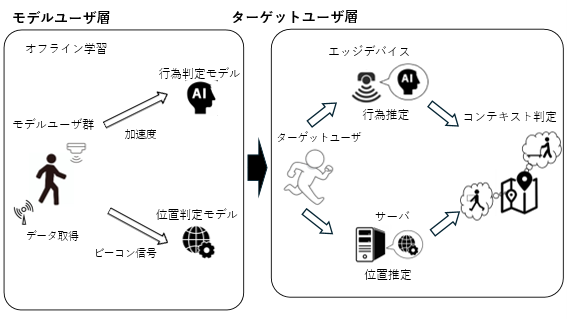
\includegraphics[width=0.8\linewidth]{Figure/pic1.png}
  \caption{手法概要図全体像}
  \label{fig:pic1}
\end{figure}


本章では, 手法のデータ取得, モデル構築, リアルタイム推定の流れを説明する. 図1は, 本研究で提案するリアルタイムコンテキスト推定手法の全体構成を示している. 本手法は, モデルユーザ層とターゲットユーザ層があり, それぞれの層で行為と位置を独立に判定もしくは推定する. 「モデルユーザ」はAI判定モデルを構築するためにデータを提供する被験者, 「ターゲットユーザ」は構築済みモデルを適用してコンテキスト判定の対象となる実運用者とする. モデルユーザとターゲットユーザを分離することで, オンライン学習とリアルタイム推定を明確に区別する. 
 
モデルユーザ層とは, オフライン学習で行動と位置を判定する層である. モデルユーザから取得したデータから推定モデルを構築し, その結果をターゲットユーザに適用することで, 実環境でのリアルタイム推定を可能とする. 行為判定では, モデルユーザの加速度データに対して弱教師あり学習を適用し, ユーザ間で共有可能な行為クラスを獲得する. 位置判定では, ビーコン信号指標に対して教師あり学習を適用し, 実施する環境ごとに位置判定モデルを構築する. 

ターゲットユーザ層は, 行為推定をエッジデバイス側, 位置推定をサーバ側で行う. 行為推定は個人に依存した行動データ内の時系列変化を主に扱う. そのため, 個人単位で完結するエッジ処理をすることで, 学習・推定対象を単純化し, リアルタイム性と実装容易性の両立を図る. 一方, 位置推定は複数ユーザに共通する空間構造を扱う問題であり, ユーザ間のデータ比較や統合が不可欠である. よって, 全体を俯瞰的に扱うために, データをサーバ側で処理し, ユーザ間比較やモデル管理を容易にする. 最終的に, 行為判定結果と位置判定結果を統合することで, ユーザのコンテキストを判定する. 本研究では, コンテキストを「何を・どこでしているか」を表す状態として定義し, 行為および位置の判定結果から逐次的に生成する. 



\section{データ取得}

本研究では, 製造・物流現場における作業者のコンテキスト推定を目的とし, 移動と作業が繰り返される作業環境を想定したデータ取得を行う. 対象作業は, 以下の２つである. 
\begin{itemize}
  \item 作業者が荷物を積載した台車を押して移動する動作
  \item 作業者が所定位置で停止し，台車から荷物を下ろす動作
\end{itemize}

これら２つの動作が交互に繰り返されるものである. 単一の行為が長時間継続するのではなく, 周期的に切り替わる点に特徴がある. このような作業構造は, 製造・物流現場において一般的であり, 本手法の設計において重要な前提条件となる. 本研究では検証のため, 複数の作業者からデータを取得する. 

コンテキスト推定には, 作業者がどのような行動を行っているのか, センサを用いて取得する必要がある. 本研究では, 作業者の身体に慣性センサを装着し, 取得される三軸加速度を用いて行動を取得する方法を提案する. 先行研究ではジャイロセンサを併用する例が多いが[2][3], 本研究では実運用を意識し, 省電力性とエッジデバイス上でのリアルタイム処理を重視したため, 電力消費やデータ量が大きいジャイロセンサは使用しない. 加速度データは, 装着姿勢や個人差の影響を低減するため, ノルム量を加えた4軸構成で扱う. 特徴量設計の目的は, 行為の意味的解釈ではなく, 行為間の相対的な運動構造の違いを捉えることである. このため, スライディングウィンドウ方式を用いて時間変化や運動強度を反映する特徴を抽出し, リアルタイム推定に適した構成とした\bibitem{Banos2014Window}. 

またコンテキスト推定には, 作業者がどこにいるかを取得する必要がある. 本研究では, 実施環境中にビーコンを複数設置, 取得される信号指標から位置を取得する方法を提案する. 複数ビーコンから得られる信号の組み合わせを特徴量とし, 教師あり学習によって位置を推定する. ビーコン信号は環境依存性が高く, 遮蔽物やレイアウト変更の影響を受けやすいため, 絶対値ではなく相対的な変化を重視する. これにより, 追加センサを必要とせず, 実環境に適応可能な位置推定を実現する. 

これらの２つの前処理は, 特徴空間の整合性を確保するため, 後述する行為ラベリング, 作業者間対応付け, ならびにリアルタイム判定において共通に適用される. 

なお, 取得されたデータは原則として未ラベルである. 行為に関するラベルは, 評価指標を算出する目的でデータ取得直後に手作業で付与しているが, 行為ラベリング処理自体には使用していない. 一方, 位置推定に関しては, ビーコン信号指標に対して教師あり学習を適用するため, 位置ラベルを教師データとして使用している. 


\subsection{加速度データの前処理}
加速度センサから取得された三軸加速度データに対し, 装着姿勢や個人差の影響を低減するため, 各軸成分に加えてノルム量を算出し, 四軸の時系列データとして扱う. ある時刻$t$のノルム量$a_{\mathrm{norm},t}$は, 三軸加速度$a_{x,t}$, $a_{y,t}$, $a_{z,t}$から次式により算出する.

\begin{equation}
a_{\mathrm{norm},t}=\sqrt{a_{x,t}^2+a_{y,t}^2+a_{z,t}^2}
\end{equation}

ほかの特徴量として, 運動の変化量を強調するため, 各軸およびノルム量に対して一次差分を計算し, 元の値と差分値を併せて用いる.

本研究では特徴量抽出にはスライディングウィンドウ方式を採用する. ウィンドウ長は64, 128, 256, 512, 1024, 2048サンプルの複数条件を設定し, 行為の時間スケールに対する影響を検証可能な構成である. スライディング幅は1サンプルとし, 隣接するウィンドウ間で大部分が重複するため行為の切り替え点に対して高い時間分解能で特徴量を更新でき, 境界付近でも状態遷移を滑らかに追跡できる. 
各ウィンドウ内において, 以下の特徴量を算出した. 
\begin{itemize}
    \item 平均
    \item 分散
    \item 周波数領域特徴量
\end{itemize}
周波数領域特徴量とは, 加速度系列に対して高速フーリエ変換（FFT）を適用して得られるスペクトルに対し, 周波数帯域$B$ごとに振幅二乗を帯域内で和として集約した値である. 帯域$B$について, 本研究では, 加速度系列を窓長$W$で分割し, 各窓に対してFFTを適用して周波数領域特徴量を算出する. サンプリング周波数を$f_s=100\,\mathrm{Hz}$とし, FFTの周波数分解能は $\Delta f=f_s/W$で与えられる. 周波数帯域は, $\Delta f$から上限$f_{\max}=25\,\mathrm{Hz}$までを対数間隔で10分割して定義した. 上限を$25\,\mathrm{Hz}$としたのは, 人の行為に関係する加速度の主要成分が低周波側に集中しやすく, それ以上の高周波成分はノイズや微小振動の影響が相対的に大きく, 行為差の識別に寄与しにくいと考えられるためである[28]. ただし, 個人差や作業環境によるスペクトル変動で$20\,\mathrm{Hz}$近傍の成分が失われることを避けるため, 本研究では文献で一般的に用いられる$20\,\mathrm{Hz}$よりも上側に余裕を持たせ, $25\,\mathrm{Hz}$までを特徴量の対象とした.

一方, FFTの結果は連続周波数ではなく「$\Delta f$刻みの離散周波数（周波数ビン）」として得られるため, 各帯域境界は最終的に周波数ビンに合わせて丸め込む. 具体的には, 各帯域の下限側は「その周波数以下で最も近いビン」, 上限側は「その周波数以上で最も近いビン」を採用し, 帯域が必ず1つ以上のビンを含むようにする. もし丸めの結果, 下限と上限が同じビンになって帯域幅が0になってしまう場合は, 上限側をさらに1ビン分だけ広げて, 最低1ビンを確保する. このビンへの丸めの影響により, 隣接する帯域が一部重複する場合がある.

以上の処理により, 各ウィンドウを単位とした特徴ベクトルを構成し, 行為ラベリング, 行為クラス割り当て, およびリアルタイム行為推定に用いる（表\ref{tab:feat_acc}）.

\begin{table}[tb]
  \centering
  \caption{加速度特徴量}
  \label{tab:feat_acc}
  \renewcommand{\arraystretch}{1.2}
  \begin{tabularx}{\linewidth}{|p{3.5cm}|p{3.0cm}|X|}
    \hline
    区分 & 項目 & 意味 \\ \hline
    基本系列 & 三軸加速度（x, y, z） & センサ座標系で取得した三軸加速度の時系列データ（単位：g） \\ \hline
    基本系列 & ノルム量（加速度合成） & 三軸を合成した加速度の大きさ。装着姿勢や個人差の影響を受けにくい指標として用いる \\ \hline
    時系列変換 & 一次差分 & 隣接サンプル間の変化量。運動の変化を強調するために導入する \\ \hline
    ウィンドウ特徴 & 平均 & スライディングウィンドウ内の平均値。動作の基線や強度の違いを表す \\ \hline
    ウィンドウ特徴 & 分散 & スライディングウィンドウ内のばらつき。振動の大きさや不規則さを表す \\ \hline
    周波数領域特徴 & 周波数帯域別パワー & FFTで得たスペクトルを周波数帯域ごとに集約した特徴量。行為に伴う周期的な運動特性を反映する \\ \hline
  \end{tabularx}
\end{table}


\subsection{ビーコン受信LQIデータの前処理}
ビーコンから取得されたデータは受信LQI（Link Quality Indicator）である. LQI は電波の受信状態を表す指標である. しばしば RSSI と同一視されるが, 算出仕様や量子化特性がデバイスに依存するため, RSSI とは区別し, 本研究ではビーコンの信号指標（受信 LQI）として扱う. ビーコンから取得される受信LQIデータは, 4台の受信点（SID）に対応する4系列の時系列データとして扱う. 受信LQIは, ビーコンごとの送信特性や設置条件, 受信環境の違いによる影響を受けやすく, そのままでは位置推定に不向きである. そこで, 時刻で時系列を整列し, 受信点（SID）ごとに受信LQIを整形した後, 未受信に対応する欠損値を補完する. 欠損値は線形補間により補完し, 系列の先頭・末尾に残る欠損については直近の観測値で補完した（前方／後方補完）. その後, 列方向のスケール変換, 行方向の相対化処理, および時間方向の処理を組み合わせた前処理を行う. 

列方向のスケール変換として, 各ビーコン列に対して二種類の正規化を適用する. 一つ目は列方向min–max正規化であり, 各ビーコン列の最小値と最大値を用いてスケーリングを行うことで, ビーコンごとの受信LQIスケールの違いを低減する. 二つ目は列方向z-score正規化であり, 各ビーコン列の平均値および標準偏差を用いて正規化することで, ビーコンごとの分布形状の差を緩和する. 

行方向の相対化処理として, 同一時刻における複数ビーコン間の相対関係を表現する特徴量を導入する. 行方向比率では, 各時刻における受信LQIの総和に対する各ビーコンの比率を算出し, 絶対的なLQIスケールに依存しない相対的な関係を表現する. また, 各時刻における受信LQIの大小関係を順位として表し, 同一時刻内でのLQIの優劣関係を行方向順位という特徴量として用いる. 

さらに, 時間方向の処理として, 各受信点系列に対して平均および差分を算出する. 時間方向平均は, 時刻順に並んだ受信サンプル列に対し, 直近10サンプルを1ウィンドウとするスライディングウィンドウ（窓幅10）で算出し, 短周期のばらつきを低減する目的で用いる. 差分は隣接サンプル間の差として定義し, 受信LQIの変化を強調する特徴量として用いる. 

以上のように, 
 \begin{itemize}
     \item 列方向のスケール変換（min–max正規化, z-score正規化）
     \item 行方向の相対化処理（比率, 順位）
     \item 時間方向の処理（平均, 差分）
 \end{itemize}
の三つの観点から前処理を行い, 位置推定モデルへの入力とする（表\ref{tab:feat_bea}）. 

\begin{table}[tb]
  \centering
  \caption{ビーコン特徴量}
  \label{tab:feat_bea}
  \renewcommand{\arraystretch}{1.2}
   \begin{tabularx}{\linewidth}{|p{3.2cm}|p{3.0cm}|X|}
    \hline
    区分 & 項目 & 意味 \\ \hline
列方向のスケール変換 & min–max 正規化 & 各ビーコン列を0–1にスケーリング \\ \hline
列方向のスケール変換 & z-score 正規化 & 各ビーコン列を平均0・分散1に正規化 \\ \hline
行方向の相対化処理 & 比率 & 同一時刻における受信LQI総和に対する各ビーコンの比率 \\ \hline
行方向の相対化処理 & 順位 & 同一時刻内の受信LQIの順位 \\ \hline
時間方向の処理 & 平均 & スライディングウィンドウで平均値 \\ \hline
時間方向の処理 & 差分 & 隣接時刻間の受信LQI変化量 \\ \hline
  \end{tabularx}
\end{table}


\section{モデルユーザからの推定モデル構築}
\begin{figure}[tb]
  \centering
  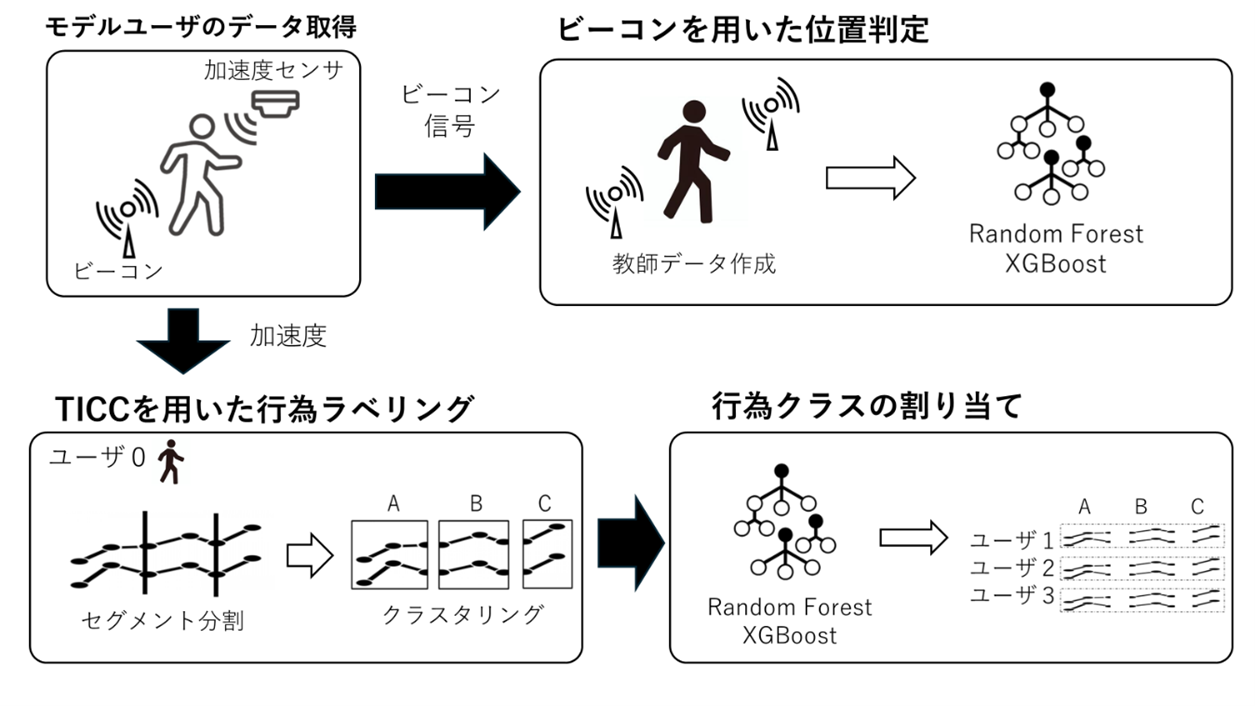
\includegraphics[width=0.8\linewidth]{Figure/pic2.png}
  \caption{モデルユーザ層内の処理}
  \label{fig:pic2}
\end{figure}

図\ref{fig:pic2}に, モデルユーザ層内の処理の流れを示す. 本図は, 実運用に先立ち, モデルユーザから行為判定および位置判定をする過程を示している. 行為判定では, モデルユーザの加速度時系列データに対して教師なしクラスタリングを適用し, 行為構造を表す行為クラスを抽出する. 行為クラスとは作業者の動作を加速度センサからの情報をもとに分類したもので, 作業の内容を機械的に分類するために使用する. その後, 抽出された行為クラスを擬似的な教師ラベルとして利用し, 他ユーザへの割り当てモデルを構築する. 一方, 位置判定では, 環境内に設置したビーコンから取得される信号指標を用い, 教師あり学習によって作業者の位置を判定する. 

モデルユーザから生成される情報は, (1)教師なしで獲得された行為クラス, (2)他作業者に対する行為クラス割り当てモデル, (3)位置推定のための教師あり学習モデルである. これらはオフライン環境下で構築され, ターゲットユーザへのリアルタイム適用時には再学習を行わない. 

本手法の特徴は, 教師なし時系列クラスタリングによってモデルユーザから獲得された行為クラスを, 後段の推定モデルにおける擬似的な教師ラベルとして利用する点にある. これにより, 人手による行為ラベリングを行うことなく, 他作業者に対する行為クラス割り当てモデルを構築できる. この二段構成により, モデルユーザが一人存在すれば, 追加の手作業による行為ラベリングを行うことなく新規データを継続的に蓄積・活用できる. さらに, 行為の意味的ラベルを事前に定義する必要がないため, 実運用環境における長期的なデータ収集およびスケーラブルな運用に適している. 

加えて, 位置判定は, ビーコン信号を用いた教師あり学習により, 環境依存性の高い位置情報を柔軟に扱える点に特徴がある. これにより, 追加センサを必要とせず, 現場のレイアウト変更にも対応可能な構成を実現している. 

\subsection{ICCを用いた行為ラベリング}
モデルユーザから取得した時系列加速度データは, そのままでは作業者の行動を表すことはできない. 行為判定モデルを構築するには, 多量の学習データと対応する正解ラベルが必要であるが, 作業現場でそれらを大規模に取得し, 一貫した基準で人手ラベル付けすることはコスト面・運用面の制約から現実的でない. さらに, 行為は単一時刻の観測値だけでは捉えられず, 時間方向の連続性や変動パターン（周期性・持続性・状態遷移）を考慮する必要がある. 前述の2種類の行為はこれらの時系列特徴が異なるため, 時系列クラスタリングによりクラスタとして分離できると考えられる. よって, 教師なし時系列クラスタリング手法であるToeplitz Inverse Covariance-based Clustering（TICC）を適用し, 行為構造を表す行為クラスを生成する\bibitem{Hallac2017}. TICCは, 時系列データをスライディングウィンドウ単位で分割し, 各区間を局所的なガウス・マルコフ過程としてモデル化することで, 時間方向の依存構造に基づいたクラスタリングを行う手法である. これにより, 行為の開始・終了や意味的ラベルを事前に定義せず, 時系列の構造そのものに基づいてクラスを獲得する. 本研究では, 前処理済みの加速度データを入力として, モデルユーザごとの2種類の分類クラスを結果として得る. 


\subsection{行為クラスの割り当て}
TICCにより得られたクラスタリング結果を行為クラスとして扱い, これを教師ラベルとして他作業者への割り当てを行う. 具体的には, 単一のモデルユーザの行為クラスを基に行為クラス番号を定義し, 分類モデルを用いて他作業者のセンサ特徴量に対応した行為クラス番号を出力する. 分類モデルには, 決定木構造を持つランダムフォレスとXGBoostの2つの分類手法\bibitem{Breiman2001}\bibitem{Chen2016}を用いる. これらの手法を採用した理由は, 少量データでも非線形な特徴量間相互作用を表現でき, バギングや正則化によりノイズ影響を抑えつつ安定した分類性能を得やすいこと, さらにスケーリング等の前処理に依存しにくく, 特徴量重要度を通じて行為クラス分離に寄与する時系列特徴を解釈しやすいことにある. 本研究では, １モデルユーザの行為クラスを他作業者へ対応付けしたクラスを, クラス割り当ての結果として得る. 


\subsection{ビーコンを用いた位置判定}
位置判定は, 行為判定とは独立に実行する. 実施環境中にビーコンを設置し, ビーコンが提供する信号指標を用いて教師データを作成する. 本研究で用いる信号指標は, 端末が出力する受信 LQIである. これらの信号は取得タイミングが不連続であり, 周囲環境や遮蔽物の影響を強く受けるという特徴を持つ. 
位置判定において教師あり学習を採用した理由は, ビーコンの設置位置や環境構成が運用環境ごとに異なるためである. 実環境では, 設置条件やレイアウトの違いにより, 環境に応じた位置推定モデルの調整が必要となる. 教師あり学習を用いることで, 各環境に対して柔軟に位置推定モデルをチューニング可能な構成を採用している. リアルタイム推定への適用を考慮し, 分類モデルとしてランダムフォレストおよびXGBoostを使用する\bibitem{Breiman2001}\bibitem{Chen2016}. これらの手法は, 推論時の計算構造が比較的単純であり, リアルタイムでの実時間処理に適している. 



\section{ターゲットユーザに対する推定モデル}
\begin{figure}[tb]
  \centering
  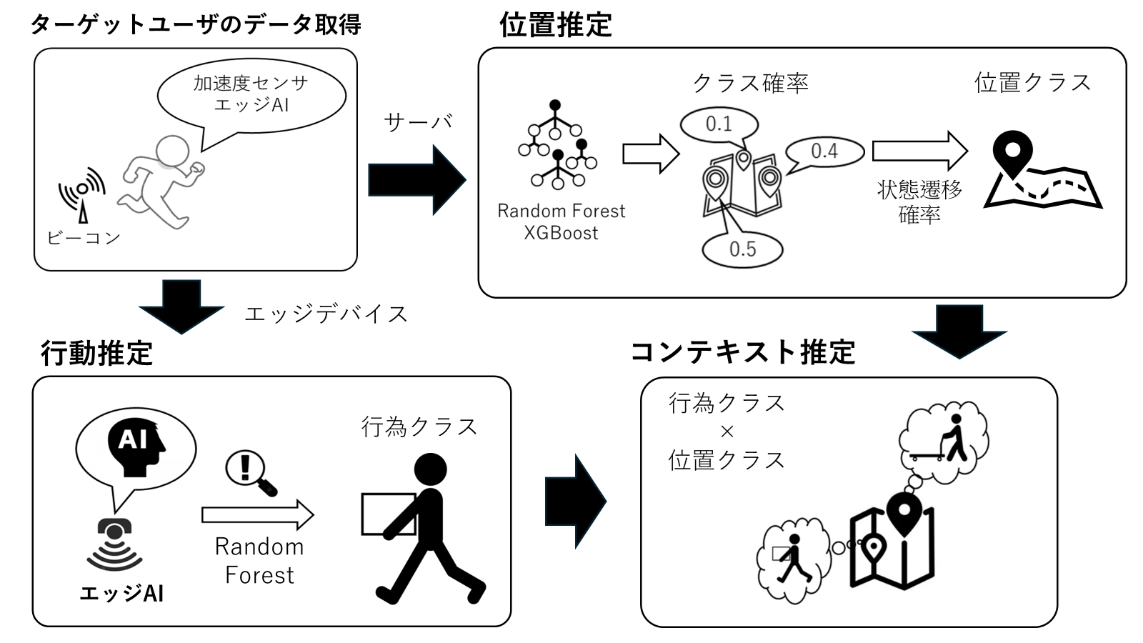
\includegraphics[width=0.8\linewidth]{Figure/pic3.png}
  \caption{ターゲットユーザ層内の処理}
  \label{fig:pic3}
\end{figure}

図\ref{fig:pic3}では, 3.2節で説明した処理構造に基づき, ターゲットユーザに対する行為および位置のリアルタイム判定を行い, それらを統合してコンテキストを推定する. 行為推定と位置推定を独立に実行し, その結果を時刻同期に基づいて統合する. 



\subsection{エッジAIによるリアルタイム行為推定}
3.2.2節で生成した行為クラスを用い, エッジデバイス上で行為推定をリアルタイムで行う. リアルタイム処理では, 入力されるセンサ時系列データに対してスライディングウィンドウを適用し, 各ウィンドウに前処理および特徴量計算を施した後, 分類モデルにより行為クラスを推定する. ここで用いる前処理および特徴量計算はオフライン処理時と同一であり, 学習時と推定時で特徴量空間の不整合が生じないよう設計している. 

ただし, エッジ実装ではハードウェア資源に制約があるため, 3.2.2節の行為割り当てモデルをそのまま搭載するのではなく, エッジ搭載を想定した軽量推定モデルを別途学習して用いる. 本研究では, モデル規模（例：決定木本数など）に制約を設けたランダムフォレストを軽量推定モデルとして採用し, 制約下での推定を可能にする. なお, 行為クラス生成から軽量推定モデル学習までの関係は図\ref{fig:pic4}に示す. 

行為推定は各スライディングウィンドウ単位で独立に実行され, 時間的変化を逐次的に追跡できる. 以上の構成により, オフラインで獲得した行為クラスに基づき, エッジデバイス上でのリアルタイム行為推定を実現する. 本研究では, 2種類の行為クラスを行為推定の結果として得る. なお, 評価時には、疑似教師ラベルではなく、実際の行動を正解ラベルとして用いる.  
\begin{figure}[tb]
  \centering
  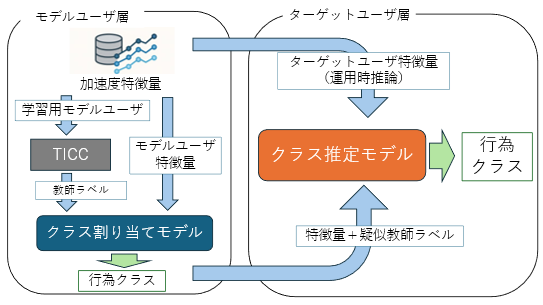
\includegraphics[width=0.8\linewidth]{Figure/pic4.png}
  \caption{行為クラス推定の流れ}
  \label{fig:pic4}
\end{figure}


\subsection{教師あり学習によるリアルタイム位置推定}
リアルタイム位置推定では, 前処理および特徴量計算は, オフライン学習時と同一である. 

しかし, 分類結果をそのまま位置判定結果として用いると, 時間的に不連続な位置の跳躍が発生する可能性がある. 実環境では被験者の位置が短時間で大きく変化することは不自然であるため, 分類モデルの出力をクラス確率として扱い, 時間方向の連続性を考慮した位置平滑化処理を行う. 各時刻において分類モデルが出力する位置クラスの確率分布を観測確率とし, 隣接する位置クラス間でのみ遷移が起こりやすいという仮定に基づいた状態遷移モデルを導入する. この遷移モデルでは, 同一位置に留まる確率を最も高く設定し, 時間的に隣接する位置クラスへの遷移のみを許容する. 

各時刻の位置推定は, 前時刻の状態確率に遷移モデルを適用して得られる予測分布と, 当該時刻の分類モデル出力確率とを統合することで更新される. この更新処理により, ノイズや一時的な誤分類の影響を低減した位置推定結果を得る. 

本研究では, 平滑化前の分類モデルの出力と, 平滑化後の出力の2種類を位置推定の結果として得る. 

\subsection{行為推定と位置推定の統合によるコンテキスト判定}
行為推定結果と位置推定結果の統合には, あらかじめ定義したルールベースの方法を用いる. 推定された行為クラスと位置クラスの組に対して, 対応するコンテキストを割り当てる. 例えば, 行為が「歩行」で位置が「廊下」の場合にはコンテキストを「移動」とし, 行為が「静止」で位置が「作業エリア」の場合には「荷下ろし」と判定する. このように, 行為と位置の意味的な組み合わせに基づく規則集合によってコンテキストを決定する. 

ルールベースの統合を採用した理由は三点ある. 第一に, 行為推定と位置推定の誤差要因を明確に分離できる点である. 第二に, コンテキストの定義は作業内容や環境構成に強く依存するため, 学習モデルに組み込むよりも, 現場に応じて柔軟に調整可能である点である. 第三に, エッジデバイス上でのリアルタイム処理を前提とした場合, 計算量および実装の簡潔さが重要となるため, ルールベース手法を用いる. 

このように, 行為推定および位置推定を独立に実行し, その結果をルールベースで統合する. 教師なしで獲得された行為構造と環境依存な位置情報を組み合わせ, 実用環境に適用可能なコンテキスト判定を行う. この目的に対し, 行為と位置の統合には, 解釈性と実装容易性を重視した手法を採用している. 



\section{評価方法}
本研究では, 行為ラベリング, 行為クラス割り当て, リアルタイム行為推定, 位置推定, およびそれらを統合したコンテキスト判定について, それぞれの処理段階の特性に応じた評価を行う. 


\subsection{行為ラベリングおよび行為クラス割り当ての評価}
\begin{enumerate}[label=(\arabic*)]
  \item 行為ラベリングの評価\\
  TICCにより得られる行為クラスは, 作業者ごとに出力結果の行為クラス番号の割当が任意であり, 同一の行為クラスであっても作業者ごとに番号が異なる. 各作業者に, 行為クラス番号に対応する番号を定義する対応付けが必要である.  この対応付けは, 行為クラス番号を行為クラスに対応させたときの一致度が最大となる割当を求めることで実施する. 本研究では対応付け後のラベル列を予測ラベルとして評価する.  なお, この対応付けは被験者間でクラスタリング性能を比較・集計するための評価用後処理であり, 運用時に行為クラスタ番号を直接行為クラスへ変換することを意図しない. 

  評価指標は, 全体正解率, 多数クラス正解率, 少数クラス正解率, およびBalanced Accuracyとする. ここで, ある時刻$t$の対応付け後の予測ラベルを$\hat{y}_t$, 正解ラベルを$y_t$とすると, 全体正解率$\mathrm{Acc}$は次式で与えられる.

\begin{equation}
f_{\mathrm{acc}}(\hat{y}_t)=
\begin{cases}
1, & \hat{y}_t=y_t,\\
0, & \text{otherwise}.
\end{cases}
\end{equation}

\begin{equation}
\mathrm{Acc}=\frac{1}{N}\sum_{t=1}^{N} f_{\mathrm{acc}}(\hat{y}_t).
\end{equation}

本指標は全データにおけるTICCによる分類結果である行為クラスと正解クラスとの一致率を示す.
2種類の行為クラスのうち, データ数が多いクラスを多数クラス, データ数が少ないクラスを少数クラスと示す. これらのクラスを識別するために多数クラスを$c_0$, 少数クラスを$c_1$とする.

多数クラスと少数クラスのそれぞれの正解率は, クラス集合を$\mathcal{C}$, 各クラス$c_n$のサンプル数を$N_{c_n}$とすると, クラス別正解率$\mathrm{Acc}_{c_n}$は次式で与えられる.

\begin{align}
\mathcal{C} &= \{c_n \mid 0 \le n \le 1\},\\
N_{c_n} &= \left|\{\,t \mid y_t=c_n\,\}\right|,\\
\mathrm{Acc}_{c_n} &= \frac{1}{N_{c_n}}\sum_{t: y_t=c_n} f_{\mathrm{acc}}(\hat{y}_t).
\end{align}

本指標はクラスごとの正解率を示す.

多数クラス正解率は$N_c$が最大となるクラスの$\mathrm{Acc}_c$, 少数クラス正解率は$N_c$が最小となるクラスの$\mathrm{Acc}_c$とする. Balanced Accuracy $\mathrm{BA}$はクラス別正解率の平均として定義する.

\begin{equation}
\mathrm{BA}=\frac{\mathrm{Acc}_{c_0}+\mathrm{Acc}_{c_1}}{2}.
\end{equation}

これはクラス不均衡の影響を受けやすい全体正解率に対し, 両クラスを同等に評価する再現率を重視した指標である. Balanced Accuracy は2値分類における感度（TPR）と特異度（TNR）の算術平均としても定義され, クラス不均衡下で両クラスを同等に扱う評価指標として用いられる[32].

本研究では, クラスタリング結果の比較（パラメータ選定）において$\mathrm{BA}$を主指標とする. これは, 行為ラベルにクラス不均衡が生じる場合, 全体正解率$\mathrm{Acc}$は多数クラスに引きずられ, 多数クラスのみを当てる解でも高く評価されうるためである. $\mathrm{BA}$は少数クラスの取りこぼしを明確に評価に反映できる. また, 多数／少数クラス正解率を併記することで, 誤りがどのクラスに偏るかを診断できる.

  \item 行為クラス割り当ての評価\\
  ターゲットユーザの行為クラス割り当てをする分類モデルは, モデルユーザに対してTICCが出力する行為クラス番号を基に分類する. よって,  分類モデルの出力と実際の行為クラスの評価をする場合, 実際の行為クラスを正解ラベルとし,  出力結果と比較には対応付けが必要である.  この対応付けは,  行為ラベリングの評価に用いたものと同一である. 評価時以外は,  分類モデルの出力は正解ラベルとなるため,  被験者ごとの追加の対応付けは行わない. 
  
評価指標には F1 スコア（macro）を用いる. 分類結果はターゲットユーザに付与する疑似ラベルとして用いられるため, 適合率も重要となる. F1は適合率と再現率の両方を反映し, かつ macro 平均によりクラス不均衡の影響を抑えて各クラスを同等に評価できるため, 本段階の目的に適合する. なお, 作業者ごとの評価に加え, 評価対象の全作業者の予測列と正解列を連結して算出した統合 F1を算出し, 全体傾向を代表する指標として用いる. 

  
\end{enumerate}

\subsection{リアルタイム推定の評価}
リアルタイム推定について, 行為判定, 位置推定, および両者を統合したコンテキスト判定の精度を評価する. 以下では, 総実施時間$T$内のある時刻$t$における行為クラスを$a_t$, 位置クラスを$l_t$とする.

\begin{enumerate}[label=(\arabic*)]
  \item リアルタイム行為推定の評価\\
  行為推定では, クラス不均衡の影響を考慮しつつ, 運用上重要となる誤検知（False Positive）と取りこぼし（False Negative）の両方を反映するため, 各行為クラスの判定性能を F1 スコアにより評価する. 本研究では各クラスを同等に扱うため F1（macro）を用いる. 

  \item リアルタイム位置推定の評価
  位置推定は, 廊下を進行方向に沿って区間（7クラス）に離散化した分類問題である. 位置クラス$l_t \in \{0,\ \ldots,\ 6\}$の区間定義は4.1.3節に示す.

位置は一次元的に連続して変化するため, 完全一致のみを正解とする評価は実用上の誤差を過大評価する場合がある. そこで, 隣接許容精度$\mathrm{Acc}_{\mathrm{loc}}$と平均絶対誤差（MAE）により評価する. ある時刻$t$の予測位置クラスを$\hat{l}_t$とすると, 隣接許容精度は, 推定クラスが正解クラスから1区間以内であれば正解とみなす指標であり, 次式で定義する.

\begin{equation}
f_{\mathrm{loc}}(\hat{l}_t)=
\begin{cases}
1, & \lvert \hat{l}_t-l_t\rvert \le 1,\\
0, & \text{otherwise}.
\end{cases}
\end{equation}

\begin{equation}
\mathrm{Acc}_{\mathrm{loc}}=\frac{1}{T}\sum_{t=1}^{T} f_{\mathrm{loc}}(\hat{l}_t).
\end{equation}

また, MAEは次式で定義する.

\begin{equation}
\mathrm{MAE}=\frac{1}{T}\sum_{t=1}^{T} \lvert \hat{l}_t-l_t\rvert .
\end{equation}

なお, 位置推定では平滑化処理を適用する場合があるため, 平滑化前後の両方について同一指標で評価し, 平滑化による改善効果を確認する.

  \item コンテキスト判定の評価
  コンテキストは行為クラスと位置クラスの組$(c_t, l_t)$として定義される. 本研究では, 行為判定は完全一致（$\hat{c}_t=y_t$）を正解とし, 位置推定は隣接許容（$\lvert \hat{l}_t-l_t\rvert \le 1$）を満たす場合を正解とみなして, 両者が同時に成立する場合のみをコンテキスト正解として評価する. このとき, コンテキスト正解率$\mathrm{Acc}_{\mathrm{ctx}}$は次式で定義される.

\begin{equation}
\mathrm{Acc}_{\mathrm{ctx}}=\frac{1}{N}\sum_{t=1}^{N}
\left( f_{\mathrm{acc}}(\hat{c}_t)\land f_{\mathrm{loc}}(\hat{l}_t) \right).
\end{equation}
\end{enumerate}

\chapter{実験}
\section{実験環境}
\subsection{使用センサ}
行為情報の取得には, トワイライト社製の慣性センサトワイライト2525Aを使用した. 本センサは三軸加速度を計測可能であり, サンプリング周波数は100Hzである. 取得された加速度データは, 10サンプルずつまとめてパケットとして送信される. 各データは, 時刻情報と三軸加速度（x, y, z）から構成される. なお, 加速度の座標系には地球座標系とセンサ座標系が存在するが, 本研究で扱う三軸加速度はセンサに固定された,  センサ座標系に基づく値である. 


センサは作業者の首後部に装着する. この位置は, 作業中の動作を妨げにくく, 身体全体の運動を安定して取得可能である. 装着姿勢は全被験者で統一しており, 加速度の各軸は, x軸を鉛直方向, y軸を左右方向, z軸を前後方向と定義する. 


位置情報の取得には, beaconviを用いた. ビーコンは合計4台設置し, 作業環境内に配置した. ビーコンの設置高さは足元付近とし, 廊下に沿って配置した. 図\ref{fig:pic5}より, 右端側から順にbeacon3, beacon2, beacon1, beacon0とした. ビーコンは廊下に沿って配置し, 隣接ビーコン間隔は約10〜20mとした. なお, 作業（タスク）は, beacon3から開始して, beacon0まで移動し, beacon3までの往復を1セットとしている. 


\begin{figure}[tb]
  \centering
  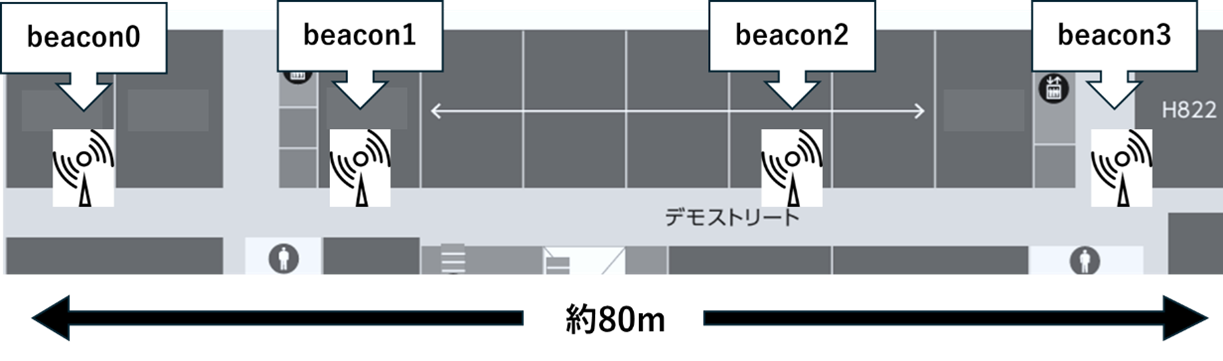
\includegraphics[width=0.8\linewidth]{Figure/pic5.png}
  \caption{ビーコン設置場所}
  \label{fig:pic5}
\end{figure}

ビーコンは動作検知時に信号を送信するため, 取得データの時間間隔は一定ではない. 各受信レコードは, PC時刻（受信時刻）, 受信中継機ID（SID）, およびリンク品質指標（LQI）から構成される（表\ref{tab:bea_data}）. 受信は作業者が携帯する端末を介して行い, 単一のPCに集約して記録した. 

\begin{table}[tb]
  \centering
  \caption{ビーコン取得データ}
  \label{tab:bea_data}
  \renewcommand{\arraystretch}{1.2}
  \begin{tabular}{|p{3cm}|p{4cm}|p{8.0cm}|}
    \hline
    区分 & 項目 & 意味 \\ \hline
時刻情報 & 時刻（PC時刻） & PCに記録された受信時刻 \\ \hline
受信点ID & 受信中継機ID（SID） & 受信に関与した中継機（受信点）の識別子 \\ \hline
受信品質 & LQI & リンク品質指標（受信品質の指標） \\ \hline
  \end{tabular}
\end{table}


\subsection{実施タスクおよび環境}
本研究では, 加速度データについては20歳から24歳の大学生13 人分（内男性7 人）の被験者データを取得した. 一方, ビーコン受信LQIデータについては, これらの被験者のうち9 人分のデータを解析対象とした. 残りの被験者については, ビーコン受信LQIが十分に取得できておらず, 位置の予測に用いるデータとして適さなかったため, 解析対象から除外した. 行為と比較して, 位置の予測は比較的少量の訓練データでも成立する問題であることから, 本研究ではこれらのデータ数で手法の有効性を検証可能であると判断した. 実験は屋内の廊下環境で実施した. 廊下の長さは約80mであり, 実験中は人通りや障害物が一部存在する環境であった. 

被験者は単独で作業を行い, 台車を押して移動し, beacon2, beacon1, beacon0 の各設置位置付近で停止して荷下ろしを行った後, 再び移動する一連の作業を実施した. この流れを1往復分行い, その間のデータを取得した. 加速度センサおよびビーコンデータは, 単一のPC上で同時に取得しており, 時刻情報は同期されている. 


\subsection{正解ラベルの付与}
本研究では, 推定結果の評価のため, 取得データに行為ラベルおよび位置ラベル（正解ラベル）を付与した. 

行為ラベルは 2 クラスとし, 台車を押して移動している状態を 0, 停止して荷下ろし作業を行っている状態を 1 と定義した. 

位置ラベルは廊下方向を一次元の位置軸として扱い, ビーコン設置位置を基準に7クラスへ離散化した. ビーコン周辺は設置位置を中心とする直径5m（前後2.5m）の区間と定義し, 隣接ビーコン間隔が約 10〜20 m であるため周辺区間は重複しない. 

各位置クラスを表\ref{tab:loc_class}に示す. 


\begin{table}[tb]
  \centering
  \caption{位置クラスの割り当て}
  \label{tab:loc_class}
  \renewcommand{\arraystretch}{1.2}
  \begin{tabular}{|p{3cm}|p{6cm}|}
  \hline
  位置クラス & 場所 \\ \hline
0 & beacon3–beacon2 間 \\ \hline
1 & beacon2 周辺（直径 5 m） \\ \hline
2 & beacon2–beacon1 間 \\ \hline
3 & beacon1 周辺（直径 5 m） \\ \hline
4 & beacon1–beacon0 間 \\ \hline
5 & beacon0 周辺（直径 5 m） \\ \hline
6 & beacon0 より左側  \\ \hline
   
  \end{tabular}
\end{table}

なお, タスクは beacon3 から開始して beacon0 まで移動し折返す往復動作を含むため, 折返し時に beacon0 を越えて左側へ進入する区間をクラス6として定義した. 

\section{得られたデータについて}
本節では, 実験により取得されたデータの特徴について述べる. 加速度センサおよびビーコンから得られるデータを用いて行為判定および位置推定を行うが, これらの前処理前のデータはそのままでは解析に適さない特性を持つ. 本節では, 代表的な1人分のデータを例として, 前処理前のデータの性質を可視化し, その特徴を示す. 

\subsection{加速度データ}
図\ref{fig:pic6}に, 1人分の三軸加速度データの時系列例を示す. 図には, 加速度センサから取得された鉛直方向（x軸）, 左右方向（y軸）, 前後方向（z軸）のデータ（単位：g）を示している. 加速度の値は, 重力加速度を基準とした$g$で表す. ここで$1\,g = 9.81\,\mathrm{m/s^2}$とし, 必要に応じて$a[\mathrm{m/s^2}]=a[g]\times 9.81$により換算できる. なお, 本データは重力成分を除去していないため, 静止時であっても姿勢に応じて各軸に重力の投影が含まれる.

\begin{figure}[tb]
  \centering
  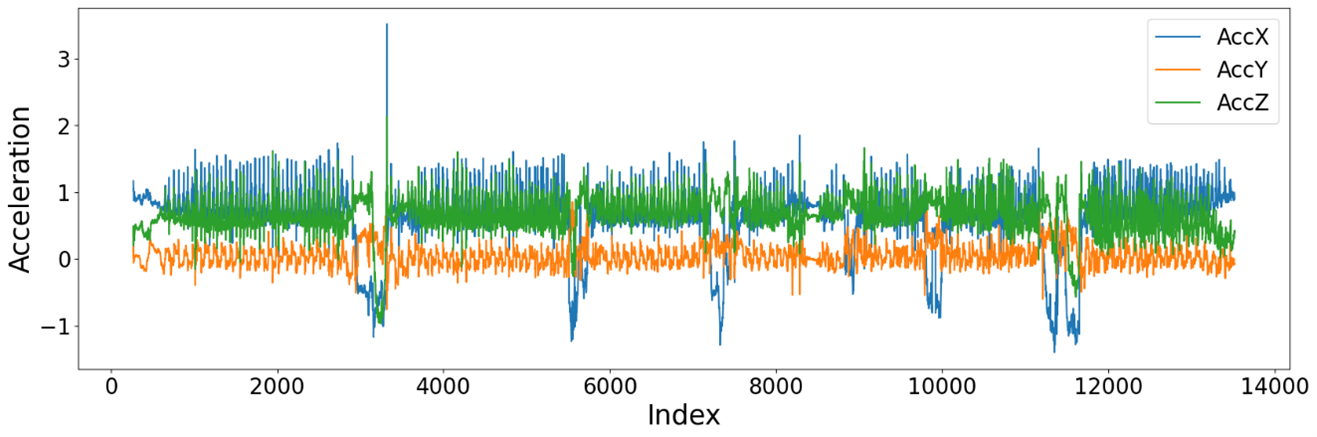
\includegraphics[width=0.8\linewidth]{Figure/pic6.png}
  \caption{取得加速度データ}
  \label{fig:pic6}
\end{figure}


\begin{table}[tb]
  \centering
  \caption{加速度データ統計量}
  \label{tab:acc_des}
  \renewcommand{\arraystretch}{1.2}
  \begin{tabular}{|l|r|r|r|}
    \hline
     & AccelerationX & AccelerationY & AccelerationZ \\ \hline
    count & 13252 & 13252 & 13252 \\ \hline
    mean  & 0.619953818 & 0.049289164 & 0.656891337 \\ \hline
    std   & 0.478859134 & 0.158544335 & 0.274429496 \\ \hline
    min   & -1.4 & -0.756 & -0.968 \\ \hline
    25\%  & 0.568 & -0.064 & 0.524 \\ \hline
    50\%  & 0.7 & 0.036 & 0.668 \\ \hline
    75\%  & 0.86 & 0.132 & 0.816 \\ \hline
    max   & 3.52 & 0.972 & 2.132 \\ \hline
  \end{tabular}
\end{table}



図\ref{fig:pic6}より, 区間0〜2750を観察すると, 三軸加速度はいずれも周期的な振動を示し, 振動の周期および振幅がおおむね一定に保たれている. この区間は実験記録上の移動時間と一致しており, 移動動作に伴う繰り返し運動が加速度波形に反映されていると解釈できる. 一方, 区間2751〜3500では, 周期的な振動が弱まり, 変動幅も小さくなる傾向が確認できる. この変化は停車して荷下ろしを行っている時間帯と一致し, 停止・作業時には移動時と比較して加速度の時間変動が抑制されることを示す. 

なお, 本データは重力成分を除去していないため, 各軸の平均値には重力加速度の投影が含まれる. 装着向きは被験者間で統一したが, 微小な傾きの差でも重力投影が変化するため, 各軸の平均値や分散には姿勢差の影響が残り得る. 表\ref{tab:acc_des}に示す要約統計より, AccelerationXとAccelerationZの平均はそれぞれ0.620g, 0.657gと0から偏る一方, AccelerationYの平均は0.049gと小さい. また, 標準偏差はX：0.479g, Y：0.159g, Z：0.274gであり, 軸ごとに変動の大きさが異なることが分かる. これらは, 装着姿勢や動作方向の違いが, 各軸の平均値および変動パターンに影響し得ることを示唆する. さらに表２より, AccelerationXは最大3.520g, 最小−1.400g（AccelerationZ最大2.132g, 最小−0.968g）を取り得ることから, 波形中に突発的なピークが含まれ, 衝撃や急な姿勢変化, 短時間の外れ値が混入している可能性がある. 

以上より, 加速度の生系列は重力投影や突発的ピークの影響を受け, 単一時刻の値に基づく比較では被験者間で分布が揺れやすい. そこで 3.1.1節で述べたように, ノルム量・一次差分に加え, スライディングウィンドウ内の統計量および周波数帯域別特徴量として集約し, 行為の時間的構造として扱う. 


\subsection{ビーコン受信LQIデータ}
図\ref{fig:pic7}に, 4.1で例示した被験者のビーコン受信LQIデータの時系列例を示す. 図\ref{fig:pic7}の横軸は時刻, 縦軸は受信LQI, 4つの折れ線グラフは4台のビーコンを示している. 

\begin{figure}[tb]
  \centering
  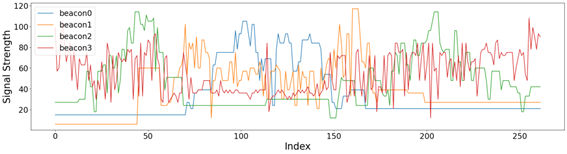
\includegraphics[width=0.8\linewidth]{Figure/pic7.png}
  \caption{取得受信LQIデータ}
  \label{fig:pic7}
\end{figure}


\begin{table}[tb]
  \centering
  \caption{受信LQI統計量}
  \label{tab:loc_des}
  \renewcommand{\arraystretch}{1.2}
  \begin{tabular}{|l|r|r|r|r|}
    \hline
 & beacon0 & beacon1 & beacon2 & beacon3 \\ \hline
count & 262 & 262 & 262 & 262 \\ \hline
mean & 34.28244275 & 39.36641221 & 47.4389313 & 55.13358779 \\ \hline
std & 25.85378125 & 24.60031651 & 25.40963426 & 20.17645572 \\ \hline
min & 15 & 6 & 12 & 12 \\ \hline
25\% & 15 & 27 & 27 & 36 \\ \hline
50\% & 21 & 36 & 42 & 48 \\ \hline
75\% & 39 & 57 & 60 & 72 \\ \hline
max & 105 & 117 & 114 & 108 \\ \hline
欠損値 & 45 & 22 & 1 & 0 \\ \hline
  \end{tabular}
\end{table}


図\ref{fig:pic7}を観察すると, 各ビーコンの受信LQIは時間とともに優勢なビーコンが入れ替わる. 特に, 受信LQIが高い区間がbeacon3 → beacon2 → beacon1 → beacon0 → beacon0 → beacon1 → beacon2 → beacon3の順で現れており, 廊下を往復移動した際に, 各ビーコン設置位置付近を通過すると対応するビーコンの受信LQIが上昇する傾向が確認できる（図\ref{fig:pic5}参照）. 

一方で, 受信LQIはビーコンごとにスケールや変動幅が異なり, 単純比較が難しい. 実際に表\ref{tab:loc_des}の要約統計では, 平均値がbeacon0：34.3, beacon1：39.4, beacon2：47.4, beacon3：55.1とビーコン間で異なり, 中央値もbeacon0：21に対してbeacon3：48と差がある. 加えて, 短時間で急激に変化する区間も存在し, 受信環境の影響を受けやすいことが分かる. また, beacon0, 1では欠損値も多数確認できる. 

以上より, 受信LQIの生系列はビーコン間のスケール差と時間的なばらつきを含み, そのまま位置推定へ入力すると不安定になる可能性がある. このため位置推定では, 未受信に起因する欠損を補完した上で, ビーコン間のスケール差を抑える正規化と, 同一時刻内の比率,  順位および時間方向処理を組み合わせ, 3.1.2節の手順に従って特徴量を構成する. 

以上より, 加速度および受信 LQI の生データは, 重力投影・外れ値・欠損・スケール差・時間的ばらつきといった要因により, そのままでは安定した推定入力になりにくい. 以降の解析では, 3章で定義した前処理・特徴量抽出を適用したデータを用いて, 行為ラベリングおよび各推定モデルの評価を行う. 



\chapter{時系列セグメントの行為ラベリング}
本章では, オフライン段階におけるTICCによる行為ラベリングと, その結果を擬似教師とした行為クラス割り当ての性能を整理する. 

\section{実験条件}
加速度データから抽出したウィンドウ単位の特徴ベクトルを入力として行う（3章表4）. 前処理, 特徴量設計, 正解ラベルの付与方法などは3章・4章の設定に準拠する. 

TICCの設定は以下の通りとする. 
\begin{itemize}
    \item window\_size = 1
    \item number\_of\_clusters = 2
    \item beta = 100
    \item maxIters = 30
\end{itemize}

※ここでいう window\_size はTICC側の設定値であり, 本章で比較する「ウィンドウ長（64〜2048）」とは別のパラメータとして扱う. 

本研究では TICC の window\_size を 1 とし, 各時刻の状態推定を 1ステップ単位で行う. 状態遷移の抑制は切り替えペナルティを与えるパラメータ beta によって制御される. beta を大きくすると状態が頻繁に切り替わりにくくなり, 短時間の外れ値に対して頑健な推定になりやすい. 一方で, 過度に大きい場合は遷移の追従が遅れ, 遷移近傍で誤りが増える可能性がある. maxItersを30とし, クラスタリング計算の試行回数を固定する. 

\section{クラスタリング結果}
スライディングウィンドウによって生成される時系列セグメントのウィンドウ長を変化させたとき, TICCによるクラスタリング性能がどのように変化するかを評価する. ウィンドウ長を以下の条件で比較する. 
\begin{itemize}
    \item ウィンドウ長：64, 128, 256, 512, 1024, 2048
    \item スライド幅：1
\end{itemize}
各条件において, 被験者ごとにTICCを適用し, クラスタリング結果を得る. 評価の際は, 被験者ごとの評価値に加え, 被験者全体の平均により全体傾向を確認する.

ウィンドウ長ごとの全被験者平均の評価結果を分析する. 表5.1に, 全体正解率$\mathrm{Acc}$, 多数クラス正解率$\mathrm{Acc}_{c_0}$, 少数クラス正解率$\mathrm{Acc}_{c_1}$, Balanced Accuracy $\mathrm{BA}$を示す. 図\ref{fig:pic8}に, 表\ref{tab:win_class}の結果を折れ線として示す. 横軸をウィンドウ長, 縦軸を各評価指標の値とする.


\begin{table}[tb]
  \centering
  \caption{クラスタリング性能の被験者平均}
  \label{tab:win_class}
  \renewcommand{\arraystretch}{1.2}
  \small
  \begin{tabular}{|l|r|r|r|r|}
    \hline
    window size &
    \makecell{全体正解率\\$\mathrm{Acc}$} &
    \makecell{多数クラス正解率\\$\mathrm{Acc}_{c_0}$} &
    \makecell{少数クラス正解率\\$\mathrm{Acc}_{c_1}$} &
    \makecell{Balanced Accuracy\\$\mathrm{BA}$} \\ \hline
    64   & 0.768 & 0.806 & 0.654 & 0.730 \\ \hline
    128  & 0.900 & 0.944 & 0.769 & 0.856 \\ \hline
    256  & 0.913 & 0.937 & 0.841 & 0.889 \\ \hline
    512  & 0.897 & 0.900 & 0.885 & 0.893 \\ \hline
    1024 & 0.852 & 0.826 & 0.933 & 0.879 \\ \hline
    2048 & 0.771 & 0.722 & 0.919 & 0.820 \\ \hline
  \end{tabular}
\end{table}

\begin{figure}[tb]
  \centering
  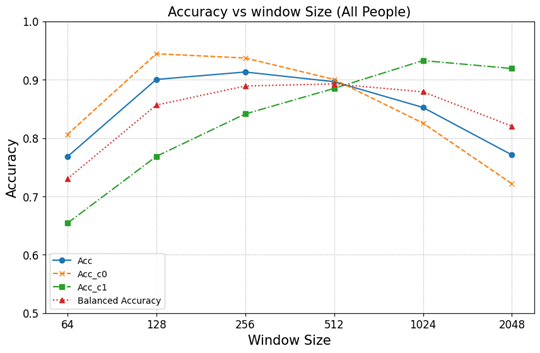
\includegraphics[width=0.8\linewidth]{Figure/pic8.png}
  \caption{ウィンドウ長とクラスタリング性能の差}
  \label{fig:pic8}
\end{figure}

表\ref{tab:win_class}および図\ref{fig:pic8}より, ウィンドウ長の変更に伴いクラスタリング性能が変化することが確認できる. 全体正解率は256で最大となり, それ以上では低下傾向がみられる. また, 多数クラス正解率も128, 256付近で高く, ウィンドウ長の増加に伴って低下する傾向がみられる. 一方で, 少数クラス正解率はウィンドウ長を大きくした条件で改善する傾向がみられ, 多数クラスとの間にトレードオフが生じることが分かる. 多数・少数の双方を同等に扱うBalanced Accuracyを確認すると, Balanced Accuracyは256と512で同程度であった. 

\begin{figure}[tb]
  \centering
  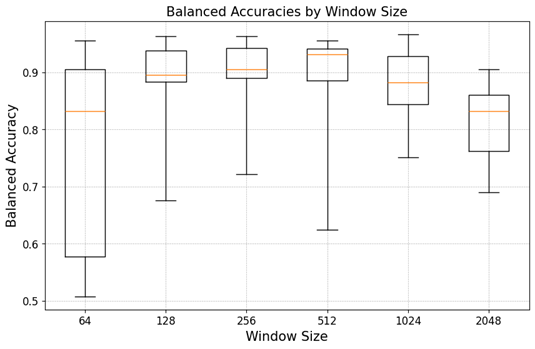
\includegraphics[width=0.8\linewidth]{Figure/pic9.png}
  \caption{被験者別精度分布}
  \label{fig:pic9}
\end{figure}

次にBAを用いて被験者ごとの違いについて分析する.  図\ref{fig:pic9}は, ウィンドウ長ごとの被験者別 Balanced Accuracy の分布を示す. 図\ref{fig:pic9}より, ウィンドウ長によって中央値とばらつきが大きく変化することが分かる. まず, 64では中央値が低く, 分布の幅も大きいことから, 短いウィンドウでは被験者間で性能が安定しにくい傾向が見られる. 一方, 128～512では中央値が高い水準にあり, クラスタリング性能が相対的に良好な条件である. さらに, 四分位範囲はいずれも比較的狭く, Balanced Accuracy の観点では安定して高いスコアを得やすいことが確認できる. 

ただし, 最小値が低い値まで伸びていることから, 一部の被験者では性能が低下している可能性がある. これは, この条件が平均的には良好である一方で, 個人差の影響を完全には吸収できていないことを示唆する. さらに, 1024では中央値の低下と, 四分位範囲の増加が確認できることから, 長いウィンドウでは特定被験者で性能が崩れる場合がある. 2048では中央値がさらに低くなり, 全体として性能が劣化する傾向が見られる. 以上より, 64のような短すぎるウィンドウは安定性に欠け, 1024以上の長すぎるウィンドウは典型性能の低下が生じやすい. 

\begin{figure}[tb]
  \centering
  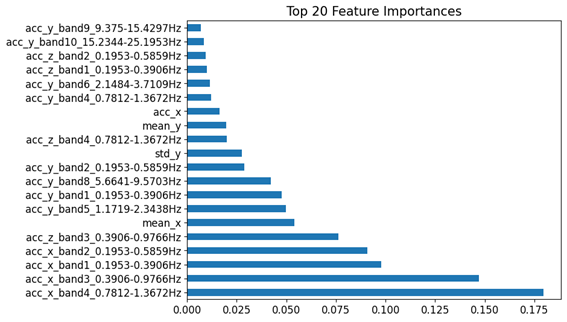
\includegraphics[width=0.8\linewidth]{Figure/pic10.png}
  \caption{上位重要変数}
  \label{fig:pic10}
\end{figure}

\begin{figure}[tb]
  \centering
  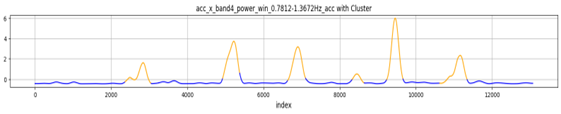
\includegraphics[width=0.8\linewidth]{Figure/pic11.png}
  \caption{重要変数（周波数帯域パワー）の時系列＋クラス色分け図}
  \label{fig:pic11}
\end{figure}

次に, ウィンドウ長を512にした場合の変数重要度を確認する. 図\ref{fig:pic10}にランダムフォレストによる被験者１の上位20位の重要変数を示す.  図より,  加速度xの特定周波数帯域パワーが上位を占めていることが確認できる. 図\ref{fig:pic11}に変数重要度が一番大きい特徴量をクラスごとに可視化する. 少数クラスで顕著なピークが繰り返し観測され, ウィンドウ内の一部の強い振動が特徴量を支配している可能性があることが分かる. 


\section{ウィンドウ長がクラスタリング性能に与える影響}
表\ref{tab:win_class}および図\ref{fig:pic8}より, ウィンドウ長の増加に伴い性能指標が一様には改善せず, 多数クラス正解率と少数クラス正解率の間にトレードオフが生じることが確認できる. ここでは, この挙動を「特徴量の推定安定性」と「ウィンドウ内の異なる行為の混在」の2点から解釈する. 

まず, ウィンドウが64の条件で性能が伸びない理由は, 被験者の局所的な挙動を多く含むため, 被験者間のばらつきが増えるためである. 実際, 被験者別の分布では短いウィンドウの時に中央値が低く, 分布幅も大きく示されている（図\ref{fig:pic9}）. 短いウィンドウでは微小なノイズや一時的な動きが特徴量に強く反映され, クラスタ間の分離が弱まりやすい. 加えて, 本研究ではFFTに基づく周波数帯域特徴量を用いているため, ウィンドウ長が短いほど周波数分解能が粗くなり, 帯域内に含まれる周波数ビン数が減少する. その結果, 帯域内の振幅集約値が観測ノイズや瞬間的な被験者の挙動の影響を受けやすくなり, 被験者間での分散が増加して推定が不安定になりやすい. 

次に, ウィンドウが1024や2048と長くなると多数クラス正解率が低下し, 少数クラス正解率が改善するという逆転現象が発生する（図\ref{fig:pic8}）.  これは, ウィンドウ内に異なる行為が混在する区間が増加する傾向と整合する. 4章の結果より, 多数クラスは約2000点程度連続で発生する一方, 少数クラスは500〜1000点程度の連続で発生する. したがってウィンドウ長が長い場合, ウィンドウ区間の内部に少数クラス区間が含まれる確率が高まり, ウィンドウ内の特徴量が単一行為に対応したものから混合的なものへ移行しやすい. 本研究で重要度が高かった特徴量は, ウィンドウ系列をFFTで周波数変換し, 周波数帯域に分割した上で, 特定帯域内の振幅を集約した値である（図\ref{fig:pic11}）. この特徴量は時間領域の局所的な形状ではなく, ウィンドウ全体の帯域成分を要約するため, 異なる行為が同一ウィンドウ内に含まれる場合, 帯域成分はそれぞれの行為に由来する周波数成分の寄与を受けた混合スペクトルとして観測される. 特に少数クラスで当該帯域成分が相対的に強い場合, 少数クラス区間がウィンドウ内に一部含まれるだけでも, 帯域特徴量が少数クラス側へ寄りやすくなる. その結果, 少数クラスに近い特徴を持つウィンドウが増加し, 少数クラス正解率は上昇する.  また, 多数クラス側では少数クラス側へ引き寄せられるウィンドウが増加し, 多数クラス正解率が低下すると解釈できる. 

最後に, 実運用におけるウィンドウ長の調整指針を述べる. ウィンドウ長はデータ処理上の都合ではなく, (1) 検出したい行為の時間スケールと, (2) 許容遅延（リアルタイム性）に基づいて決めるべきである. 本実験では少数クラスが500〜1000点程度連続して発生する.  よって,  ウィンドウ長は少数クラス区間を一定割合以上含みつつ, ウィンドウ内に異なる行為が混在する区間を過度に増やさない範囲に設定することが望ましい. この観点から, 本研究の設定範囲では, 短すぎる64では推定が不安定になりやすく, 長すぎる1024以上では混在の影響が増加しやすい. 本研究の加速度データは100Hzで取得しているため, 512のような中間的なウィンドウ長は約5秒の観測区間に相当し, 少数クラス区間の一部を含みつつ混在の増加を抑えやすいという点で, 両者のトレードオフを取りやすい. 

以上より, ウィンドウ長はクラスタリング性能に影響を与える設計変数であることが確認できる. 以降の行為クラス割り当て評価では, 本節の全体傾向と被験者間ばらつきを踏まえ, Balanced Accuracy の観点で不利になりにくく, かつトレードオフを考慮して, 少数クラスの再現性を確保しやすい条件としてウィンドウ長を 512 に固定する. 


\section{クラス割り当ての結果}
クラスタリング結果を擬似教師として学習した分類モデルが, 他被験者に対して同一の行為クラスをどの程度安定して割り当てられるかを評価する. なお本評価では, 5.3節の結果を踏まえ, Balanced Accuracy の観点で不利になりにくく, かつ少数クラスの再現性を確保しやすい条件として, ウィンドウ長を 512 に固定する. 
\begin{itemize}
    \item ウィンドウ長：512
    \item スライド幅：1
\end{itemize}
割り当てモデルとして Random Forest（RF）および XGBoost（XGB）を用い, 訓練者を入れ替えながら評価した. 評価指標は訓練者データ1人に対するクラスタリング性能としてクラスタリングF1スコア, 他被験者に対する割り当て結果の性能として統合 F1を用いる. 

\begin{table}[tb]
  \centering
  \caption{訓練者ごとのクラスタリングF1, RF・XGBによる統合F1}
  \label{tab:tr_class_F1}
  \renewcommand{\arraystretch}{1.2}
  \small
  \begin{tabular}{|l|r|r|r|}
    \hline
    被験者 & クラスタリングF1スコア & RF　統合F1 & XGB　統合F1 \\ \hline
被験者１ & 0.943 & 0.632 & 0.757 \\ \hline
被験者２ & 0.913 & 0.725 & 0.756 \\ \hline
被験者３ & 0.942 & 0.743 & 0.787 \\ \hline
被験者４ & 0.948 & 0.785 & 0.738 \\ \hline
被験者５ & 0.959 & 0.783 & 0.774 \\ \hline
被験者６ & 0.835 & 0.755 & 0.794 \\ \hline
被験者７ & 0.929 & 0.738 & 0.752 \\ \hline
被験者８ & 0.898 & 0.829 & 0.817 \\ \hline
被験者９ & 0.738 & 0.804 & 0.8 \\ \hline
被験者１０ & 0.916 & 0.774 & 0.772 \\ \hline
被験者１１ & 0.83 & 0.738 & 0.805 \\ \hline
被験者１２ & 0.907 & 0.65 & 0.744 \\ \hline
被験者１３ & 0.899 & 0.667 & 0.729 \\ \hline
平均 & 0.897 & 0.74 & 0.771 \\ \hline
標準偏差 & 0.059 & 0.057 & 0.027 \\ \hline
  \end{tabular}
\end{table}


表\ref{tab:tr_class_F1}より, 訓練者によって割り当て性能が変動することが確認できる. また, 同一訓練者に対してRFとXGBを比較すると, 平均統合F1はXGBがRFを上回る一方, 訓練者によってはRFが同等または上回る場合もみられる. 
次に, 訓練者ごとの割り当て性能のモデル差を可視化するため, 訓練者ごとの統合F1を棒グラフとして 図\ref{fig:pic12}に示す. 

\begin{figure}[tb]
  \centering
  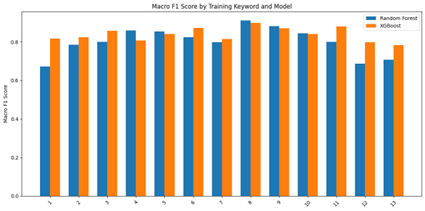
\includegraphics[width=0.8\linewidth]{Figure/pic12.png}
  \caption{訓練者×モデルの統合F1}
  \label{fig:pic12}
\end{figure}

図\ref{fig:pic12}より, 訓練者に依存した性能差が存在し, またRFとXGBで性能傾向が必ずしも一致しないことが分かる. 

さらに, 訓練者のクラスタリング性能と割り当て性能の関係を確認するため, クラスタリングF1スコアとRF, XGBの統合F1の散布図を図\ref{fig:pic13_pic14}に示す. 

\begin{figure}[tb]
  \centering
  \begin{minipage}{0.48\linewidth}
    \centering
    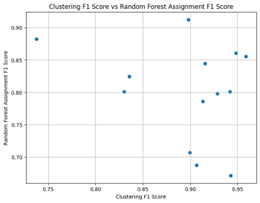
\includegraphics[width=\linewidth]{Figure/pic13.png}
    \subcaption*{RF}
  \end{minipage}\hfill
  \begin{minipage}{0.48\linewidth}
    \centering
    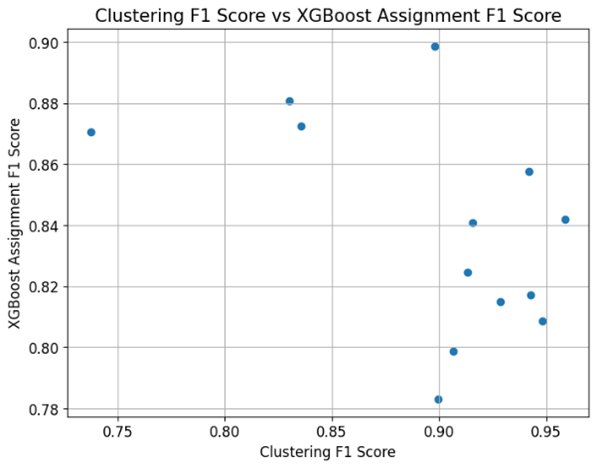
\includegraphics[width=\linewidth]{Figure/pic14.png}
    \subcaption*{XGB}
  \end{minipage}
  \caption{クラスタリングF1×割り当てF1}
  \label{fig:pic13_pic14}
\end{figure}

図\ref{fig:pic13_pic14}より, クラスタリングF1が高い訓練者ほど割り当て性能も高い, という単調な関係は明確ではなく, 訓練者によってばらつきがみられる. 

\section{行為クラス割り当てにおけるモデル選定と訓練者依存}
5. 4節では, 訓練者1人のクラスタ結果を教師ラベルとして他被験者へ割り当てる設定を取り, RFおよびXGBで統合F1を評価した. その結果, 訓練者の選択により割り当て性能が変動し, またモデル間でも傾向が一致しないケースが確認できる. 平均と標準偏差を見ると, XGBはRFよりも平均性能が高く, ばらつきも小さく安定という傾向がある. このことは, 被験者間の分布ずれが存在する条件下では, XGBの方が境界を柔軟に表現でき, 訓練者に依存した性能の落ち込みが相対的に小さくなる可能性を示唆する. 一方で, 特定の訓練者ではRFが同等以上となる場合もあり, 単純にモデルだけで一意に決まる問題ではない. 

さらに, クラスタリングF1と割り当て性能の関係を図5. 4で確認すると, クラスタリングF1が高い訓練者ほど割り当ても高いという単調関係は明確でない. これは, 訓練者本人のクラスタ分離が良いことと, 他者に一般化可能な判別規則が得られることが別物であるためである. つまり, 割り当て性能は「訓練者のクラスタがどれだけ典型的か」, 「他者の特徴分布とどれだけ重なるか」に強く依存し, クラスタリングF1だけでは決めきれない. 

以上を踏まえると, 本研究の条件では, (1) 割り当てモデルとしては平均性能と安定性の観点からXGBを第一候補としつつ, (2) 訓練者の選定はクラスタリングF1のみで判断せず, 統合F1の実測に基づいて行う, とするのがいいと考えられる. 



\chapter{エッジAIによるリアルタイム行為推定}
本章では,  ターゲットユーザ層のエッジAIを用いたリアルタイム行為推定について整理する. 

リアルタイム行動推定で学習に用いる教師ラベルは,  モデルユーザ層の行為判定モデルで作成した行為クラスである. 行為クラスは, 5章の訓練者入れ替え評価において最もクラス割り当て性能が高い被験者8を訓練とし、ランダムフォレストで分類した設定により得られた割り当て結果を採用する. これらを, 推定精度の評価は３章で定義した指標に従い, 正解ラベルに対して算出する. 

\section{実験条件}
5章と同様に, 加速度データから生成する特徴ベクトルを入力として行う（表\ref{tab:feat_acc}）. 本章の各評価に共通する条件を以下に示す.  
\begin{itemize}
    \item スライディングウィンドウのスライド幅は1で固定
    \item 学習に用いるラベルは, 5章で作成した行為ラベル
    \item 評価の正解ラベルは, 実際の行動
    \item 分類モデルにはランダムフォレスト（RF）
\end{itemize}



\section{決定木の本数による推定精度変化}
決定木の本数が推定精度に与える影響を確認するため, RFの決定木の本数を4本, 10本, 100本として比較する. 12人をモデルユーザ, 1人をターゲットユーザとする条件で比較する.

まず, 被験者13人を順にターゲットユーザとし, 他12人をモデルユーザとし, パラメータ$n\_estimators$により決定木の本数を変更して検証する.

n\_estimatorsごとの結果を表\ref{tab:num_tree_F1}に示す. 平均F1スコアは$n\_estimators=4$で0.885, $n\_estimators=10$で0.892, $n\_estimators=100$で0.902であり, 平均値としては決定木本数の増加に伴いわずかに上昇した. $n\_estimators=4$から$n\_estimators=10$の改善幅は$+0.0068$, $n\_estimators=10$から$n\_estimators=100$の改善幅は$+0.0103$となる. また, 標準偏差は0.041～0.044程度であることを確認した. 本条件では決定木本数増加による精度は上昇しているが, 限定的である.

図\ref{fig:pic15}にターゲットユーザごとのF1スコアを示す. 縦軸にF1スコア, 横軸にテスト対象者番号を示す. ターゲットユーザ別に見ると, 決定木本数の増加により改善が見られる被験者が存在する一方で, 条件間の差が小さい被験者や, 木本数を増やしても明確な改善が見られない被験者も確認できる. なお, 被験者8をターゲットユーザにした場合が最高精度になっているが, 被験者8がモデルユーザの行動クラスの基になっていることが原因と考えられる.


\begin{table}[tb]
  \centering
  \caption{決定木本数ごとのF1スコア}
  \label{tab:num_tree_F1}
  \renewcommand{\arraystretch}{1.2}
  \small
  \begin{tabular}{|l|r|r|r|r|}
    \hline
    $n\_estimators$ & F1（平均） & F1（標準偏差） & F1（最小値） & F1（最大値） \\ \hline
4 & 0.885 & 0.0442 & 0.7783 & 0.9418 \\ \hline
10 & 0.8918 & 0.0444 & 0.7832 & 0.9472 \\ \hline
100 & 0.9021 & 0.041 & 0.7966 & 0.953 \\ \hline
  \end{tabular}
\end{table}

\begin{figure}[tb]
  \centering
  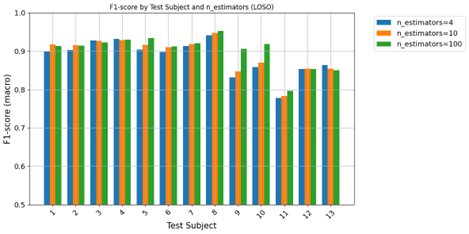
\includegraphics[width=0.8\linewidth]{Figure/pic15.png}
  \caption{テスト対象ごとのF1スコアと決定木本数の関係}
  \label{fig:pic15}
\end{figure}


\section{決定木の本数の結果に関する考察}
6.2節の結果では, 決定木の本数を増やしても性能差が小さく, ばらつきの低下も見られない. 

これは, 本研究の行為推定は2クラス分類であり, クラス間の分離が比較的容易であった可能性がある. また, 学習データ量が十分であったため, 各決定木が学習する識別境界が安定しやすく, 平均化による分散低減の追加効果が小さかった可能性を示す. さらに, 5章の分析より周波数成分が分類に強く寄与する傾向が確認されている. よって, 少数の特徴量が予測に大きく貢献している場合, 少数の決定木でも一定の精度が得られ, 決定木の本数を増やした際の改善幅が小さくなることが考えられる. 

しかし,  RF をエッジデバイス上でリアルタイムに繰り返し推定へ用いる場合, 決定木の本数には限りがある. 単一コア MCU では RF 推論は決定木を逐次に実行するループとして実装され, 推論遅延・消費エネルギは概ね決定木の本数に比例して増加することが報告されている\bibitem{Daghero2021}. さらに, 実際の運用を考慮すると, 推論を所定時間内に完了させる必要があり, 埋込み実装においても 1 ms 未満での状態推定を満たすべきである. よって, 特徴計算と分類の合計時間をサンプリング窓内に収める設計が求められる\bibitem{Kuppers2019}.  

以上より, $n\_estimators=100$は限定的ではあるが精度改善が得られる一方で, 推論コストが増大しやすい. 本研究では, 推定モデルの軽量性を優先しつつ,  $n\_estimators=4$より一貫して高い平均性能を示した設定として $n\_estimators=10$を採用する.  


\section{モデルユーザの人数による推定精度の変化}
モデルユーザの人数が推定精度に与える影響を確認するため,  モデルユーザ人数を $k$人（$k=1,\ 2,\ 3,\ 5,\ 8,\ 12$）として比較する. 決定木の本数は6.2節の結果に基づき $n\_estimators=10$に固定し,  モデルユーザの人数$k$を変化させたときのF1スコアを評価する. ターゲットユーザには各被験者を順に用いた. 各ターゲットユーザに対してランダムに選んだ$k$人をモデルユーザとして20回検証をした. それぞれの組み合わせで学習・推定を行い, 得られたF1スコアをモデルユーザの人数ごとに平均を求めた. 

表\ref{tab:num_k_F1}に, モデルユーザの人数ごとの推定精度を示す. ここで表\ref{tab:num_k_F1}のF1スコアは, 被験者13人に対して, 20通りの組み合わせで得られた260個の（13×20）平均と標準偏差を表す. 

図\ref{fig:pic16}は, 表2の平均F1スコアを図として示したものである. 平均F1スコアはモデルユーザの人数の増加に伴い単調に上昇した. また, $k=1$ から $k=2$ へは0.021の増加と改善幅が大きい一方で, その後は $k$ の増加に伴い改善幅が小さくなる傾向が見られる. F1スコアの標準偏差は, モデルユーザの人数を増やすことで推定結果のばらつきが抑えられていること分かる.  


\begin{table}[tb]
  \centering
  \caption{モデルユーザ人数$k$ごとの推定精度}
  \label{tab:num_k_F1}
  \renewcommand{\arraystretch}{1.2}
  \small
  \begin{tabular}{|l|r|r|}
    \hline
    モデルユーザ人数k & F1（平均） & F1（標準偏差） \\ \hline
1 & 0.855 & 0.057 \\ \hline
2 & 0.876 & 0.049 \\ \hline
3 & 0.885 & 0.045 \\ \hline
5 & 0.89 & 0.043 \\ \hline
8 & 0.893 & 0.044 \\ \hline
12 & 0.895 & 0.042 \\ \hline
  \end{tabular}
\end{table}

\begin{figure}[tb]
  \centering
  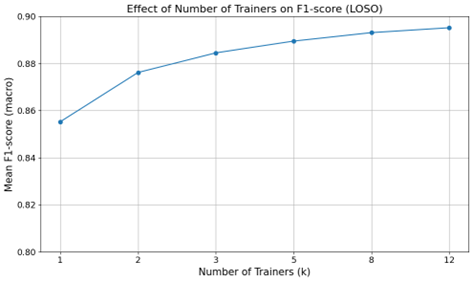
\includegraphics[width=0.8\linewidth]{Figure/pic16.png}
  \caption{モデルユーザ人数 k と平均F1スコアの関係}
  \label{fig:pic16}
\end{figure}

\section{モデルユーザの人数の増加が推定精度に与える影響}

6.4節の結果より, F1スコアはモデルユーザの人数kの増加に伴い上昇し, 標準偏差は$k=8$ではわずかに増加するが, 全体としては低下する傾向が確認できる. 標準偏差の低下は, F1スコアのばらつきが小さくなったことを示し, 推定がより安定化したことを意味する. これは, モデルユーザを増やすことで学習データが増加し, モデルユーザ間の変動を含むより広い分布を学習できるため, 特定個人に依存した偏りが緩和された可能性がある. 

一方で, $k$が大きくなるほど改善幅が小さくなる点は, モデルユーザを追加しても学習に寄与する新規情報が次第に限定的になることを示唆する. すなわち, 新たに追加されるモデルユーザがもたらす特徴が, 既に含まれているモデルユーザの特徴と重複しやすく, 性能の上積みが小さくなったと解釈できる. これは「被験者間の違いが存在しない」ことを意味するのではなく, 限られた人数の追加では, モデルが獲得できる判別境界の改善が飽和しやすいことを示す. 

また, 改善が頭打ちになる原因として, 本研究の教師ラベルがクラスタリング結果に基づく行為クラスであることも考えられる. 訓練データ量を増やしてもラベルの曖昧さや誤りが残る可能性がある. したがって, 改善幅の縮小は, モデルユーザの追加によって得られる特徴量の分布の違いが次第に限定的になる点に加え, 教師ラベルの行為クラスの不確かさが残る点の双方が影響した可能性がある.  




\section{ターゲットユーザ対象者による推定精度の変化}

次にターゲットユーザによる推定精度のばらつきと個人差の関係について分析する. モデルユーザの人数を$k=12$に固定し, 決定木の本数は$n\_estimators=10$とした条件で, ターゲットユーザを入れ替えて評価する.  

表\ref{tab:test_F1}に, 被験者のF1スコアの高い順で示す. $k=12$, $n\_estimators=10$の学習条件において, 全体としては高い推定精度が得られている一方で, 被験者によって推定精度に差が見られる. 最も高い被験者ではF1スコアが0.947, 最も低い被験者では0.783であり, 両者の差は約0.16であった. 

表\ref{tab:test10_F1}に, 最も低い推定精度を示した被験者10の指標を示す. 被験者10ではAccuracyが0.835, F1スコアが0.783であった. また少数クラスであるクラス1に着目すると, $precision=0.62$, $recall=0.74$, $F1=0.68$であった.  

\begin{table}[tb]
  \centering
  \caption{被験者ごとのF1スコア}
  \label{tab:test_F1}
  \renewcommand{\arraystretch}{1.2}
  \small
  \begin{tabular}{|l|r|}
    \hline
    テスト対象者番号 & F1 \\ \hline
8 & 0.9472 \\ \hline
4 & 0.929 \\ \hline
3 & 0.9268 \\ \hline
7 & 0.9192 \\ \hline
1 & 0.9175 \\ \hline
5 & 0.9164 \\ \hline
2 & 0.9159 \\ \hline
6 & 0.9107 \\ \hline
10 & 0.87 \\ \hline
12 & 0.855 \\ \hline
13 & 0.8542 \\ \hline
9 & 0.8478 \\ \hline
11 & 0.7832 \\ \hline
  \end{tabular}
\end{table}

\begin{table}[tb]
  \centering
  \caption{被験者10のクラス別指標}
  \label{tab:test10_F1}
  \renewcommand{\arraystretch}{1.2}
  \small
  \begin{tabular}{|l|r|r|r|r|}
    \hline
   クラス & support & precision & recall & F1 \\ \hline
0 & 9374 & 0.92 & 0.86 & 0.89 \\ \hline
1 & 2866 & 0.62 & 0.74 & 0.68 \\ \hline
marco avg & 12240 & 0.77 & 0.8 & 0.78 \\ \hline
  \end{tabular}
\end{table}

\section{個人差が残ることの意味}
6.6節の結果より, ターゲットユーザ対象者によって推定精度に差が残ることが確認できる. すなわち, 本研究の設定では, 全体として高い推定精度が得られる状況であっても, 特定の被験者に対しては推定性能が相対的に低下し得る. このことは, ターゲットユーザ対象者の違いが性能を左右する要因として無視できないことを示している. したがって, エッジ推定を適用したリアルタイム行為推定では, 平均精度だけでなく, ターゲットユーザによって精度が低下し得る点を前提として評価・設計を行う必要がある. 

6.6節で最も低い推定精度を示した被験者10では, 少数クラス（クラス1）のprecision の低下が見られ, 誤検出が増加している. この背景として, 本研究ではセンサ装着部位・向きを統一しているものの, 装着のわずかなずれや姿勢, 歩行, 作業手順の違いにより観測特徴が変化し得る点が挙げられる. これにより, 本来クラス0である区間でもクラス1に近い特徴が現れ, 学習済みの決定境界を越えてクラス1として出力されることで誤検出が増加した可能性がある. 特に本研究では周波数成分が識別に強く寄与する傾向が確認されているため, テンポや振幅の個人差が周波数特徴へ直接反映され, クラス間の分離が弱まることで誤検出が増えやすくなったと考えられる. 

図\ref{fig:pic17}および図\ref{fig:pic18}に被験者10の変数重要度が1番高い変数の時系列を示す. 図より, 予測ラベルはクラス1の区間全体にわたり安定して出力されるのではなく, 特徴量が大きく変動する箇所に断続的に出力される傾向が見られる. このことは, 当該特徴量が定常的な行為の継続よりも遷移（開始・停止）に伴う変化へ強く反応していることを示唆する. 遷移に対応するピークが判別の手がかりとなる場合, クラス1の区間が分断されやすいだけでなく, クラス0側でも同様のピークが生じた際に誤検出が増えるため, precision 低下につながり得る. なお, このずれはスライディングウィンドウで算出した特徴量とラベル付与時刻の差により見かけ上増大する可能性もある. 

以上より, 本研究で観測された個人差は, 単なる平均精度の差ではなく, 装着状態・姿勢・作業様式の差に起因する観測特徴の変形と, その結果として生じる誤検出の増加として現れる場合がある. 


\begin{figure}[tb]
  \centering
  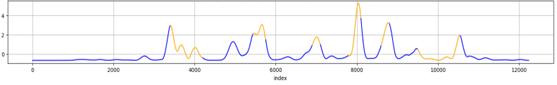
\includegraphics[width=0.8\linewidth]{Figure/pic17.png}
  \caption{正解ラベルで色分けした重要変数時系列（acc\_x\_band4\_power,0.78–1.37Hz）}
  \label{fig:pic17}
\end{figure}


\begin{figure}[tb]
  \centering
  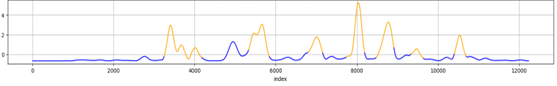
\includegraphics[width=0.8\linewidth]{Figure/pic18.png}
  \caption{予測ラベルで色分けした重要変数時系列（同上）}
  \label{fig:pic18}
\end{figure}

また, 6.4節ではモデルユーザの人数を増やすことで平均精度と安定性が改善する傾向が確認された一方, 6.6節ではモデルユーザの人数を最大限に増やした条件でもターゲットユーザ間の差が残った. したがって, 本研究で観測された個人差は, モデルユーザの人数の増加のみでは吸収しきれない要因が存在することを示唆する. 運用上は, 平均精度が高い条件であっても, ターゲットユーザによって誤検出または見落としが増加し得る点を考慮し, 要求に応じた評価指標の設定や閾値設計を行う必要がある. 

さらに, 本研究では, 5章の訓練者入れ替え評価においてクラス割り当て性能が最も高かった被験者8を基準とし, その割り当て結果を学習ラベルとして採用した。被験者8が最高値ではあるものの, 被験者3・4など同程度に高いF1スコアを示す被験者も存在する. このことは, 「擬似教師として他者へ整合しやすい」ことと, 「他者の情報を基に分類しやすい」ことが必ずしも一致しない可能性を示唆する。
以上より, リアルタイム行為推定では, 平均精度の向上だけでなく, ターゲットユーザによって性能が低下し得る点を前提として評価・設計を行う必要がある。



\chapter{ビーコン電波強度を用いた位置推定}
本章では, 受信LQIから抽出した特徴量を入力として, 位置クラスを推定する判定モデルを構築し, モデルユーザで学習したモデルをターゲットユーザへ適用する枠組みを扱う. ただし, 本研究でリアルタイム位置推定として用いる出力は判定モデル単体ではなく, 判定モデルの出力に状態遷移に基づく平滑化を組み合わせた結果である. 評価指標は3章で定義した隣接許容精度$\mathrm{Acc}_{\mathrm{loc}}$および$\mathrm{MAE}$を用いる.

本章で得られる位置推定結果は, 後段のコンテキスト判定において行為推定結果と統合する位置情報として用いる.

\section{平滑化}
本研究では, 受信 LQI から位置クラスを出力する分類モデルを位置判定モデルとして使用する. この位置判定モデルからの出力を各位置クラスの尤度として, 位置平滑化の機構に通すことでリアルタイム位置推定として使用する. 

ターゲットユーザへの推定モデルの適用時には, 前時刻の推定分布に状態遷移行列を適用して得られる事前分布と, 現時刻の観測尤度をクラスごとに統合し, softmax関数を通すことで現時刻の推定位置クラスを得る. 本章ではこの平滑化がどのような影響を結果に与えるのかを分析する. 


\section{1人学習クロスバリデーションの結果}
モデルユーザで学習した位置判定モデルをターゲットユーザへ適用する条件において, 平滑化の有無を比較する. 被験者10人のうち1人をモデルユーザとして学習し, 残り9人をターゲットユーザとして推定する. モデルユーザを入れ替えて全員分実施する. 表\ref{tab:RF_Acc}および表\ref{tab:XGB_Acc}に, モデルユーザごとのターゲットユーザ9人分の評価値を平均した結果を示す. 


\begin{table}[tb]
  \centering
  \caption{ランダムフォレストによる結果}
  \label{tab:RF_Acc}
  \renewcommand{\arraystretch}{1.2}
  \small
  \begin{tabular}{|l|r|r|r|r|}
    \hline
モデルユーザ & 判定モデル$\mathrm{Acc}_{\mathrm{loc}}$ & 推定モデル$\mathrm{Acc}_{\mathrm{loc}}$ & 判定モデルMAE & 推定モデルMAE \\ \hline
被験者１ & 0.728 & 0.763 & 0.965 & 0.843 \\ \hline
被験者２ & 0.729 & 0.766 & 1.015 & 0.901 \\ \hline
被験者３ & 0.748 & 0.817 & 0.946 & 0.737 \\ \hline
被験者４ & 0.787 & 0.825 & 0.854 & 0.771 \\ \hline
被験者５ & 0.71 & 0.745 & 1.024 & 0.974 \\ \hline
被験者６ & 0.765 & 0.844 & 0.86 & 0.696 \\ \hline
被験者７ & 0.751 & 0.786 & 0.929 & 0.798 \\ \hline
被験者８ & 0.738 & 0.773 & 0.959 & 0.841 \\ \hline
被験者９ & 0.709 & 0.737 & 0.988 & 0.891 \\ \hline
被験者１０ & 0.741 & 0.743 & 0.886 & 0.879 \\ \hline
平均 & 0.741 & 0.78 & 0.942 & 0.833 \\ \hline
標準偏差 & 0.024 & 0.037 & 0.06 & 0.084 \\ \hline
  \end{tabular}
\end{table}

\begin{table}[tb]
  \centering
  \caption{XGBoostによる結果}
  \label{tab:XGB_Acc}
  \renewcommand{\arraystretch}{1.2}
  \small
  \begin{tabular}{|l|r|r|r|r|}
    \hline
モデルユーザ & 判定モデル$\mathrm{Acc}_{\mathrm{loc}}$ & 推定モデル$\mathrm{Acc}_{\mathrm{loc}}$ & 判定モデルMAE & 推定モデルMAE \\ \hline
被験者１ & 0.741 & 0.765 & 0.954 & 0.868 \\ \hline
被験者２ & 0.713 & 0.788 & 1.008 & 0.812 \\ \hline
被験者３ & 0.77 & 0.864 & 0.929 & 0.659 \\ \hline
被験者４ & 0.78 & 0.816 & 0.873 & 0.812 \\ \hline
被験者５ & 0.697 & 0.757 & 1.253 & 1.03 \\ \hline
被験者６ & 0.748 & 0.797 & 0.982 & 0.892 \\ \hline
被験者７ & 0.729 & 0.739 & 1.002 & 0.992 \\ \hline
被験者８ & 0.723 & 0.736 & 1.012 & 0.913 \\ \hline
被験者９ & 0.691 & 0.704 & 1.099 & 1.033 \\ \hline
被験者１０ & 0.744 & 0.746 & 0.925 & 0.878 \\ \hline
平均 & 0.734 & 0.771 & 1.004 & 0.889 \\ \hline
標準偏差 & 0.029 & 0.046 & 0.107 & 0.114 \\ \hline
  \end{tabular}
\end{table}

表\ref{tab:RF_Acc}および表\ref{tab:RF_Acc}から, 平滑化を含めた推定モデルでは$\mathrm{Acc}_{\mathrm{loc}}$が増加し, $\mathrm{MAE}$が低下する傾向が確認できる. さらに, 推定モデルであってもモデルユーザにより性能に幅があり, 1人学習条件ではモデルユーザの選択が推定性能に影響しうる.


\begin{figure}[tb]
  \centering
  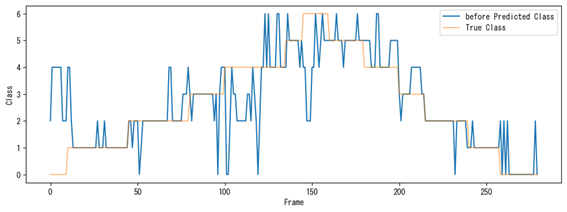
\includegraphics[width=0.8\linewidth]{Figure/pic19.png}
  \caption{判定モデルのクラス推移}
  \label{fig:pic19}
\end{figure}

\begin{figure}[tb]
  \centering
  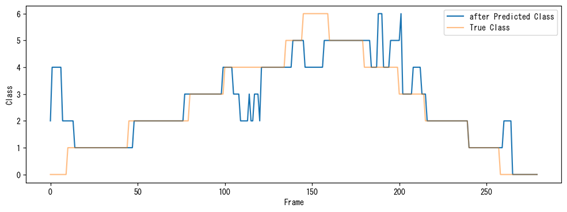
\includegraphics[width=0.8\linewidth]{Figure/pic20.png}
  \caption{推定モデルのクラス推移}
  \label{fig:pic20}
\end{figure}

図\ref{fig:pic19}, 図\ref{fig:pic20}は, モデルユーザ8で学習したRFの出力を, ターゲットユーザ10に適用したときのクラス推移である. 例示は, 図7.1の組合せのうち, 推定モデルの$\mathrm{Acc}_{\mathrm{loc}}$が平均付近となる組合せを選び, 平滑化が不連続な推定を抑える挙動を可視化する目的で示す. 判定モデルでは短時間の大きな変動を含み, 隣接しないクラスへの跳躍が散発的に生じている. 一方, 推定モデルでは推定クラスが段階的に変化し, 急激な上下動が抑制されている.


\section{位置平滑化の影響}
状態遷移に基づく平滑化は, モデルユーザで学習した位置判定モデルをターゲットユーザへ適用する際に, 推定系列の不連続を抑えて実用上の安定性を確保するための処理である. 実験結果より, 単一時刻の推定はビーコン電波強度の一時的な変動の影響を受けやすいことが分かる. しかし, 平滑化は短時間の大きな跳躍のような不連続な推定を抑制でき, 推定クラスの時間的整合性を高めることが確認できた. 

一方で, 平滑化は急な位置変化を起こりにくくする性質を持つため, 区間境界を跨ぐタイミングなど真値が切り替わる状況では追従の遅れが生じる可能性がある. また, 遷移確率の設定によって推定の挙動は変化し, 自己遷移を過度に大きくすると安定性は増すが変化点の反映が遅れる. したがって, 平滑化処理は, 推定の安定化と変化点追従のトレードオフを調整する機構として位置づけられる. 


\section{モデルユーザの違いによる位置推定精度}
表\ref{tab:RF_Acc}および表\ref{tab:XGB_Acc}は, モデルユーザごとの平均性能を示すが, ターゲットユーザごとの変動は読み取りにくい. そこで, 推定モデルの隣接許容精度を, モデルユーザごとにヒートマップとして可視化する.

図\ref{fig:pic21}および図\ref{fig:pic22}は, 縦軸をモデルユーザ, 横軸をターゲットユーザとして, 各組合せにおける推定モデルの$\mathrm{Acc}_{\mathrm{loc}}$を示したヒートマップである. これにより, モデルユーザとターゲットユーザの組合せに依存して性能が変動する様子を俯瞰できる. これらの図より, モデルユーザを固定した場合でもターゲットユーザによって精度が異なることが分かる. また, 同一のターゲットユーザに対してもモデルユーザにより精度が変動している様子が視覚的に示唆される.

\begin{figure}[tb]
  \centering
  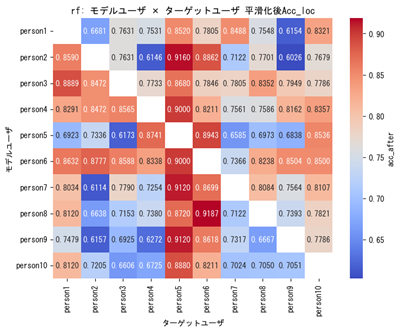
\includegraphics[width=0.8\linewidth]{Figure/pic21.png}
  \caption{RF ヒートマップ}
  \label{fig:pic21}
\end{figure}

\begin{figure}[tb]
  \centering
  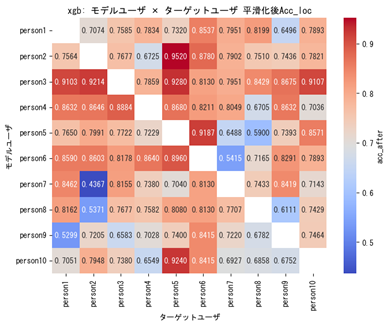
\includegraphics[width=0.8\linewidth]{Figure/pic22.png}
  \caption{ZGB ヒートマップ}
  \label{fig:pic22}
\end{figure}

表\ref{tab:target_loc}はターゲットユーザ別に隣接許容精度の平均を算出したものである. RFとXGBの両方で被験者５および被験者６が上位となっている. 一方で, 下位となる被験者はモデルにより一部異なり, XGBでは被験者8が0.722で最小であったのに対し, RFでは被験者9が0.729と最小であった. 


\begin{table}[tb]
  \centering
  \caption{ターゲットユーザごとの隣接許容精度（推定モデル）}
  \label{tab:target_loc}
  \renewcommand{\arraystretch}{1.2}
  \small
  \begin{tabular}{|l|r|r|}
    \hline
ターゲットユーザ & $\mathrm{Acc}_{\mathrm{loc}}$（RF） & $\mathrm{Acc}_{\mathrm{loc}}$（XGB） \\ \hline
被験者１ & 0.812 & 0.783 \\ \hline
被験者２ & 0.732 & 0.738 \\ \hline
被験者３ & 0.745 & 0.776 \\ \hline
被験者４ & 0.735 & 0.743 \\ \hline
被験者５ & 0.891 & 0.839 \\ \hline
被験者６ & 0.849 & 0.844 \\ \hline
被験者７ & 0.738 & 0.729 \\ \hline
被験者８ & 0.758 & 0.722 \\ \hline
被験者９ & 0.729 & 0.758 \\ \hline
被験者１０ & 0.81 & 0.782 \\ \hline
平均 & 0.7799 & 0.7714 \\ \hline
標準偏差 & 0.054229973 & 0.040556627 \\ \hline
  \end{tabular}
\end{table}

\section{モデルユーザの選定とターゲットユーザの適性}
7.4節の結果から, モデルユーザとターゲットユーザの組み合わせによって推定精度が変化するのが確認できた. よって推定精度を向上させるモデルユーザとしての適性と, 推定対象として高精度が得られやすい傾向を整理する.

モデルユーザ別平均（表\ref{tab:RF_Acc}, 表\ref{tab:XGB_Acc}）に基づき, 推定モデル$\mathrm{Acc}_{\mathrm{loc}}$を主指標としてモデルユーザの順位を確認する. RFでは被験者6, 被験者4, 被験者3が上位となり, XGBでも被験者3, 被験者4, 被験者6が上位となった. すなわち被験者3, 4, 6はモデルによらず上位に位置し, モデルユーザとして高精度になりやすい傾向が数値的に確認できる.

ただし, $\mathrm{Acc}_{\mathrm{loc}}$は隣接クラスを許容する指標であるため, 誤差の大きさも把握する観点として推定モデル$\mathrm{MAE}$も併せて確認する. 被験者3および被験者4は, RFで推定モデル$\mathrm{MAE}$がそれぞれ0.737, 0.771であり, XGBでも0.659, 0.812と相対的に低い値をとる. 一方, 被験者6はRFでは推定モデル$\mathrm{MAE}$が0.696と低い値であるが, XGBでは0.892で平均付近であり, $\mathrm{MAE}$の観点ではモデル依存の差が残る.

一方で, 低性能となるモデルユーザは両モデルで一致しており, 推定モデル$\mathrm{Acc}_{\mathrm{loc}}$はRFおよびXGBのいずれにおいても被験者9が最小となる. このことから, 被験者9をモデルユーザとした場合に位置推定精度が低下しやすい要因が存在する可能性がある. また, ターゲットユーザ側については, 表\ref{tab:target_loc}から, 被験者5, 6は両モデルで相対的に高い値となっている.

以上の整理より, $\mathrm{Acc}_{\mathrm{loc}}$の観点から被験者6はモデルユーザとして両モデルで上位に位置し, かつターゲットユーザとしても高い値をとるため, 被験者6を位置推定における代表例として便宜上用いる. 代表モデルユーザが高精度となる要因として, 受信系列の欠損が少なく観測が安定している可能性がある. ただし, 代表モデルユーザである被験者6を用いた場合でも, 被験者7に対しては精度が大きく低下する組み合わせが確認された（RF：0.7366, XGB：0.5415）. この低下要因として, 実験時の人や遮蔽物の配置といった周囲環境の差により電波伝搬条件が変化し, 受信LQIの変動が増大した可能性がある. 平均性能が高いモデルユーザであっても組み合わせ依存のばらつきが残ることが示唆される.

また, 図\ref{fig:pic21}および図\ref{fig:pic22}の精度分布は, 特定の領域が一様に高い／低いといった単純なパターンにはならず, 組み合わせや測定条件に依存してばらつく可能性がある. これは, ビーコン受信LQIが測定環境の変動を受けやすいことが一因として考えられる. さらに, RFとXGBの結果は全体傾向として大きく乖離しておらず, モデル差よりもモデルユーザ・組み合わせといったデータ条件の影響が相対的に大きい可能性がある.

\section{モデルユーザの数による推定性能の変化}
7.5節より, 1人学習条件ではモデルユーザの選択によって推定性能が変動することが分かった.  よって学習データ数を増やした場合の推定性能の変化を確認する. 表\ref{tab:num_model_loc}に, モデルユーザを1〜9人に変化させたときの平均評価値を示す. 図\ref{fig:pic23_pic24}, \ref{fig:pic25_pic26}には, 表\ref{tab:num_model_loc}の隣接許容精度とMAEの推移をモデル別に示す. 

\begin{table}[tb]
  \centering
  \caption{モデルユーザ数と位置推定性能の関係}
  \label{tab:num_model_loc}
  \renewcommand{\arraystretch}{1.15}
  \small
  \begin{tabular}{|l|r|r|r|r|r|}
    \hline
    model &
    \makecell{モデル\\ユーザ数} &
    \makecell{判定モデル\\$\mathrm{Acc}_{\mathrm{loc}}$} &
    \makecell{推定モデル\\$\mathrm{Acc}_{\mathrm{loc}}$} &
    \makecell{判定モデル\\$\mathrm{MAE}$} &
    \makecell{推定モデル\\$\mathrm{MAE}$} \\ \hline

    \multirow{9}{*}{ランダムフォレスト} & 1 & 0.769 & 0.803 & 0.84 & 0.74 \\ \cline{2-6}
     & 2 & 0.783 & 0.827 & 0.79 & 0.66 \\ \cline{2-6}
     & 3 & 0.793 & 0.836 & 0.75 & 0.63 \\ \cline{2-6}
     & 4 & 0.797 & 0.842 & 0.73 & 0.60 \\ \cline{2-6}
     & 5 & 0.801 & 0.847 & 0.72 & 0.58 \\ \cline{2-6}
     & 6 & 0.806 & 0.852 & 0.70 & 0.56 \\ \cline{2-6}
     & 7 & 0.810 & 0.858 & 0.69 & 0.55 \\ \cline{2-6}
     & 8 & 0.810 & 0.861 & 0.68 & 0.54 \\ \cline{2-6}
     & 9 & 0.813 & 0.871 & 0.68 & 0.51 \\ \hline

    \multirow{9}{*}{XGBoost} & 1 & 0.753 & 0.803 & 0.91 & 0.79 \\ \cline{2-6}
     & 2 & 0.790 & 0.846 & 0.77 & 0.64 \\ \cline{2-6}
     & 3 & 0.806 & 0.860 & 0.71 & 0.59 \\ \cline{2-6}
     & 4 & 0.816 & 0.870 & 0.68 & 0.56 \\ \cline{2-6}
     & 5 & 0.823 & 0.875 & 0.65 & 0.54 \\ \cline{2-6}
     & 6 & 0.828 & 0.880 & 0.64 & 0.52 \\ \cline{2-6}
     & 7 & 0.832 & 0.884 & 0.62 & 0.51 \\ \cline{2-6}
     & 8 & 0.834 & 0.885 & 0.61 & 0.50 \\ \cline{2-6}
     & 9 & 0.833 & 0.888 & 0.61 & 0.49 \\ \hline
  \end{tabular}
\end{table}



\begin{figure}[tb]
  \centering
  \begin{minipage}{0.48\linewidth}
    \centering
    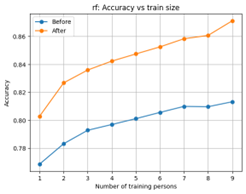
\includegraphics[width=\linewidth]{Figure/pic23.png}
    \subcaption*{RF}
  \end{minipage}\hfill
  \begin{minipage}{0.48\linewidth}
    \centering
    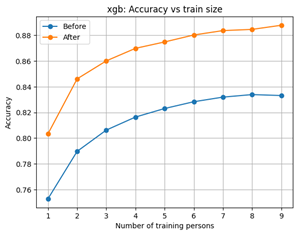
\includegraphics[width=\linewidth]{Figure/pic24.png}
    \subcaption*{XGB}
  \end{minipage}
  \caption{モデルユーザ数と精度の推移}
  \label{fig:pic23_pic24}
\end{figure}

\begin{figure}[tb]
  \centering
  \begin{minipage}{0.48\linewidth}
    \centering
    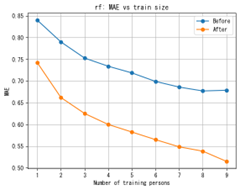
\includegraphics[width=\linewidth]{Figure/pic25.png}
    \subcaption*{RF}
  \end{minipage}\hfill
  \begin{minipage}{0.48\linewidth}
    \centering
    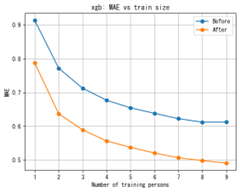
\includegraphics[width=\linewidth]{Figure/pic26.png}
    \subcaption*{XGB}
  \end{minipage}
  \caption{モデルユーザ数とMAEの推移}
  \label{fig:pic25_pic26}
\end{figure}

表\ref{tab:num_model_loc}より, モデルユーザの数の増加に伴い, RFおよびXGBのいずれにおいても隣接許容精度は増加し, MAEは低下する傾向が確認できる. 例えばモデルユーザ数を1人から5人へ増やすことで, 推定モデルのMAEはRFで 0.16, XGBで 0.25 低下し, 推定モデルの隣接許容精度はRFで +0.044, XGBで +0.072 向上した. なお, モデルユーザ数が9人の条件ではターゲットユーザの対象が1人となるため, 評価の分散が大きく, 安定しにくい可能性がある. 


\section{モデルユーザ数の影響と訓練人数の目安}
モデルユーザの数を増やした場合の推定性能の変化を整理する. 表\ref{tab:num_model_loc}および図\ref{fig:pic23_pic24}, \ref{fig:pic25_pic26}より, モデルユーザの数の増加に伴い, RFおよびXGBのいずれにおいても隣接許容精度は上昇し, MAEは低下する傾向が確認できる. 

モデルユーザの数の増加に伴い性能は概ね向上するが, 本節の設定ではモデルユーザの数が増えるほどターゲットユーザの数が減少し, 評価値が少数の被験者に強く依存する. 特にモデルユーザ数9ではターゲットユーザの対象が1人であるため, 評価値はその1人の難易度に左右され, 上振れ・下振れが生じやすい. したがって, モデルユーザ数8→9における改善は, 追加学習の効果に加えて, ターゲットユーザの対象の入れ替わりによる見かけの変動を含む可能性がある. したがって, モデルユーザ数が大きい条件の数値をそのまま比較して結論づけることには注意が必要である. 

以上を踏まえると, モデルユーザ数が少ない領域においても性能改善が得られている点が重要である. 図\ref{fig:pic23_pic24}, \ref{fig:pic25_pic26}の推移からも, モデルユーザ数4〜5人付近で改善が緩やかになる傾向が見られる. よって, モデルユーザ数4〜5人程度を実用上の1つの目安として扱うべきである. 



\chapter{コンテキスト判定}
本章では, 6章の行為推定結果と7章の位置推定結果を統合し, コンテキスト判定を行う. コンテキストの定義および評価指標は第３章で述べた方法に従う. 

\section{統合方法}
行為推定結果と位置推定結果はサンプリング周期が異なるため, 同一時刻の推定値として対応付ける必要がある. 本研究では位置推定結果の時刻を基準時刻とし, 行為推定結果の時刻から基準時刻以前で最も近い推定値を割り当てた. 未来参照による情報漏洩を避けるため, 割当は基準時刻より後の推定値を用いない. 許容時刻差は 1 秒とし, 許容差内に割り当てられない位置時刻は評価対象から除外した. 
本条件では, 全被験者合計で位置点の 3. 56\% が結合不能として除外され, 残りを評価に用いた. 

\section{評価設定}
行為推定と位置推定の両方のデータが揃う8被験者を対象に評価を行った. 各系列について, 時刻同期後に得られたデータ点数を評価母数とし, 被験者別の結果と系列平均を算出した. 

\section{結果}
表\ref{tab:context}に, 被験者別の同期後データ点数, 行為正解率, 位置正解率, およびコンテキスト精度を示す. 同期後データ点数は被験者間で約200点台であり, 各被験者の評価は同程度の母数で比較できる. 


\begin{table}[tb]
  \centering
  \caption{コンテキスト評価結果}
  \label{tab:context}
  \renewcommand{\arraystretch}{1.2}
  \small
  \begin{tabular}{|l|r|r|r|r|}
    \hline
被験者 & 同期後データ点 & 行為正解率 & 位置正解率 & コンテキスト精度 \\ \hline
被験者1 & 226 & 0.96 & 0.916 & 0.881 \\ \hline
被験者2 & 213 & 0.831 & 0.85 & 0.681 \\ \hline
被験者3 & 241 & 0.946 & 0.959 & 0.905 \\ \hline
被験者4 & 236 & 0.809 & 0.919 & 0.729 \\ \hline
被験者5 & 222 & 0.887 & 0.838 & 0.748 \\ \hline
被験者6 & 279 & 0.796 & 0.824 & 0.652 \\ \hline
被験者7 & 198 & 0.864 & 0.813 & 0.682 \\ \hline
被験者8 & 255 & 0.898 & 0.843 & 0.749 \\ \hline
平均 & 233.75 & 0.874 & 0.87 & 0.753 \\ \hline
  \end{tabular}
\end{table}

表\ref{tab:context}より, コンテキスト精度の平均は 0.753 であった. 被験者別のコンテキスト精度は 0.652〜0.905 の範囲に分布し, 個人差が確認された. 


\section{考察}
コンテキスト精度は行為推定と位置推定の同時正解を要するため, 行為正解率および位置正解率が高い場合でも, コンテキスト精度はそれらより低い値になりやすい. 実際に表\ref{tab:context}では, 行為正解率（平均0.874）および位置正解率（平均0.870）に対し, コンテキスト精度は平均0.753であった. ここで, 行為推定と位置推定の誤りが独立であると仮定すると, 同時正解率の期待値は 0.874×0.870≒0.760 となり, 実測との差は約0.007と小さい. したがって, 本結果における精度低下の主因は同時正解であり, 両者の誤りが強く同時に発生して大きく崩れている可能性は高くない. ただし, 同期処理により, 同時正解率がわずかに低下しうる点には留意が必要である. 

また, 被験者別の結果から, コンテキスト精度のばらつきは, 行為推定と位置推定のどちらが主要因となって精度を押し下げるかが被験者により異なることに対応している. 例えば, 被験者2および被験者6では行為正解率が相対的に低く, コンテキスト精度も低い. 一方, 被験者7では位置正解率が相対的に低く, コンテキスト精度の低下に寄与している. なお, 被験者間の差（0.652～0.905）は無視できない. したがって, コンテキスト精度を改善するには, 統合段階の工夫に加え, 行為推定および位置推定の誤り要因を個別に低減することが重要である. 


\chapter{本研究の限界}

本研究は, 加速度センサに基づく行為推定と, ビーコン受信情報に基づく位置推定を独立に行い, 両者の組としてコンテキストを判定する枠組みを採用した. この構成により, 行為と位置をそれぞれ適した方法で推定できる. 一方で, 推定精度および実運用を見据えた成立性には一定の限界が存在する. 


\section{個人差による識別精度の限界}
加速度センサから得られる時系列データは個人差があり, 行為推定の精度に影響を与える. 個人差には, 身長, 歩幅などの身体特性や, 台車操作の仕方, 上体の揺れ方などの作業癖が含まれる. これらの違いは, 同一の行為であっても加速度波形の振幅や周波数成分の分布を変化させ, 特徴量の類似度を低下させ得る. 例えば, 台車移動において小刻み歩行と大股歩行では, 支配的な周期成分が異なり, 周波数帯域特徴や統計量の分布が変化する可能性がある. 

センサの装着状態の差も無視できない. 装着位置の数cmのずれ, 装着角度の微小な違い, 固定具合の差は, 加速度の観測に系統的な変形を与える. 固定が緩い場合, 身体運動に対してセンサの相対運動が生じ, 余分な揺れや衝撃が観測値に混入してピークが増大することがある. 一方で, 固定具が緩衝材として働くと, 高周波の衝撃成分が減衰し, ピークが小さく観測される場合もある. すなわち, 装着差はピーク振幅と周波数成分の双方を変化させ得る. このような装着差は, 行為間差よりも大きな分布差として現れる場合があり, 推定精度低下の要因となる. 

本研究は行為推定および位置推定のどちらにおいてもモデルユーザのクラスタリング結果を教師として他者への一般化を試みる構造を含む. このとき, モデルユーザにとって妥当なクラスタ境界が, 他者に対して必ずしも妥当とは限らない. したがって, 本モデルの構造では, 分類モデルの選択や調整のみでは吸収しきれない一般化の限界が生じる. 

以上の点より, 作業者の個人差は本研究のモデル全体の識別精度の低下に作用する. よって, 実施段階では、センサの装着について手順の標準化と状態のチェックを行い, 観測段階での個人差を抑制する必要がある. 取得データに対しては, 6.5節の結果より, モデルユーザを増やすことによる特定個人の偏りを緩和する必要がある. 



\section{実験環境と実環境の乖離}
本研究では, 行為クラスおよび位置クラスを離散ラベルとして定義し, 正解ラベルに対する一致率として推定性能を評価する. しかし, 現場の状態は連続的で多様であり, それを少数の離散ラベルにまとめると, 状態の細かな違いが失われる.

本研究の行為クラスについては, 台車を押す/荷下ろしの2クラスで定義している. しかし「荷下ろし」には, 持ち上げ, 屈む, 置く, 待機といった異なる運動が含まれ, それぞれで加速度の時間変動や衝撃の出方が異なる. これは台車を押す場合も同様である. 一方で, 本研究の位置クラスは位置情報によって7クラスに定義されている. 7.3節の結果より, 位置クラスの推定結果は位置平滑化を行わない場合精度が下がる. これは, 多数クラスを分類する場合, コンテキスト判定においては連続性を考慮しないといけないことを示している. よって, 現場の状態に合わせて, 連続的で多様なラベルを用いる場合, 行為判定および行為推定の精度は下がってしまう. これは位置クラスが増えた場合も同様である. 

以上の点より, クラス数が増える場合は、連続性を考慮すべきであるということがわかる. よって, 行為においても, 平滑化処理などを用いて不連続なクラスの遷移を抑制し, 識別精度を高める必要がある. 

\section{エッジデバイス上での実装に伴う計算資源・遅延制約}
本研究はリアルタイム推定を想定し, エッジデバイスで行為推定を行う. しかし, エッジデバイスには計算資源と記憶資源の制約があり, 採用可能なモデル規模や特徴量設計が限定される. 一般に, モデルや特徴量計算を高次化すれば精度向上が期待できる一方で, メモリ消費と推論時間が増大し, リアルタイム性を満たしにくくなる. したがって, 精度とリアルタイム性の間にはトレードオフが存在し, エッジデバイス上での実装では一定の妥協が不可避である. 

具体的には, 特徴量計算を増やすほど計算量が増え, ウィンドウ長を長くするほど入力が確定するまでの待ち時間が増えるため推定遅延が増大する. また, 平滑化や履歴参照を導入すれば推定の安定性は向上し得るが, 追加の状態管理や計算が必要となり, リアルタイム性の要求を満たす条件は厳しくなる. よって, 実装先の端末性能に応じて達成可能な遅延と精度の上限は変化し得る. 

さらに, エッジAIの普及には, 推定精度以外の運用上のハードルも存在する. 現場に配備される端末の性能や仕様が統一されない場合, 搭載可能なモデル容量や許容できる遅延が端末ごとに異なる. これにより, 同一条件で学習済み推定モデルの配布, 運用することが難しくなる. 

以上より, エッジAIは計算資源の制約に加え, リアルタイム性と運用管理の両面で限界を持つ. よって, 運用環境に応じて、精度とリアルタイム性のどちらを優先するべきかを選択するべきである. また, 特徴量の選別およびパラメータ調整によるモデルの軽量化も考えられる. 

\section{ビーコン受信情報に内在する物理的限界}
位置推定は, ビーコンから得られる受信指標を入力として位置クラスを推定する. しかし, 受信指標は距離の直接観測ではなく, 電波伝搬の影響を強く受けるため, 値の安定性に限界がある. 具体的には, 遮蔽物や人体遮蔽, 反射によるマルチパスの影響により, 同一位置であっても受信値が大きく変動し得る. 

また, ビーコンから得られる受信値には欠損が多く含まれる. 欠損が多い区間では補完値が入力の一部を占めるため, 推定は実測よりも補完処理に依存しやすくなる. 特定ビーコンの欠損が長く続く場合, 利用できる識別情報が構造的に減少し, 推定の不確かさが増大する. 

以上より, 受信値の短期的な揺らぎと欠損は, 位置推定性能を低下させる. この限界を軽減するには, ビーコン配置と設置条件の最適化, 平滑化の導入により、欠損値や変動を減らす必要がある. 



\chapter{おわりに}
本研究の目的は, 行為推定や位置推定を単独で扱うだけでは作業者の状況把握に直結しにくいという課題に対し, コンテキストを「位置クラスと行為クラスの組」として定義し, 推定結果を「どこで, 何をしているか」として解釈可能にすることである. 既存の統合手法は前提に依存しやすく, また統合は位置と行為の同時正解を要するため, 本研究では行為推定と位置推定を独立に設計し, 時刻同期により統合する枠組みを採用した. 

この目的の下で, 行為については無ラベル時系列から行為クラスを生成し, 他被験者へ付与して学習へ接続する手順を構築した. さらに, 付与した行為クラスを教師情報として, エッジ実装を想定した軽量分類モデルによりリアルタイム行為推定を行った. 位置については, 受信LQI系列を特徴量化して教師あり分類を行い, 時間方向の連続性を仮定した平滑化により不自然な遷移を抑制した. 最後に, 行為推定結果と位置推定結果を時刻対応付けし, 同時正解によりコンテキスト精度を評価した. 

行為クラス生成では，無ラベル時系列から得た行為クラスを擬似ラベルとして後段の学習へ接続するため，少数クラスを含めて安定した状態列が得られるウィンドウ長条件を比較した. 複数条件を比較した結果，多数クラスと少数クラスを等重みで評価するBalanced Accuracyはウィンドウ長512で高く，0.893であった. 以上より，本研究の行為クラス生成では512を基準条件として扱えることを確認した. 

行為クラス割り当てでは，モデルユーザで生成した行為クラスを他被験者へ付与し，リアルタイム行為推定の教師情報として利用できるかを検証した. 統合F1を指標として比較した結果，被験者平均ではXGBがRFを上回った. 一方で，訓練者の選択により同一手法でも性能が変動し，割り当て性能が訓練者選択に依存しうることが確認された. 以上より，行為クラス生成の良否だけでなく，他者に対して整合しやすい行為クラスを与えられるかが行為推定の成立条件となる. さらに，モデルユーザ人数kの増加に伴い平均F1は上昇したが，改善幅は縮小しており，モデルユーザ数を増やすだけでは個人差を完全には吸収できないことも示唆された. 

位置推定では，ビーコン受信LQIに基づく位置クラス推定に対して，時間方向の連続性を仮定した平滑化を導入し，不自然な遷移を抑制できるかを評価した. 結果として，平滑化の導入により隣接許容精度は向上し，位置推定が安定化する傾向が確認された. 一方で，モデルユーザとターゲットユーザの組み合わせにより推定性能が大きく変動する例も観測され，受信環境差に起因する不安定性が残ることが示唆された. さらに，モデルユーザ数を増やすことで改善傾向は見られたが，変動を完全には解消できなかった. 

コンテキスト判定では，行為推定と位置推定を独立に実行した上で，同一時刻における両者の組を用いて「位置クラス×行為クラス」として状況を判定し，同時正解により評価した. 結果として，被験者平均のコンテキスト精度は0.753であった. 以上より，本設定では同時正解を要するという条件がコンテキスト精度を左右しやすく，行為推定と位置推定の両方を安定化させることが統合精度の改善に直結することを確認した. 

今後の課題は, 個人差と装着差を前提とした一般化性能の改善, 擬似ラベルの品質管理と他者整合性の向上, 受信環境変動と欠損に対する位置推定の頑健化, ならびにエッジ実装における計算資源と遅延制約を踏まえた軽量化に整理される. また, 現場の状態は連続的で多様であるため, 連続性を考慮した平滑化や確率的統合への拡張も重要である. 

以上より, 無ラベル時系列から行為クラスを生成してリアルタイム行為推定へ接続する手順, およびLQIに基づく位置推定に時間方向の整合を組み込む手順は, いずれも有効性が確認できた. さらに, 行為推定結果と位置推定結果を同一時刻で統合することで, コンテキストを「位置クラスと行為クラスの組」として判定できることを示した. この枠組みは, 作業者の状態を継続的に把握する必要がある一方で, 人手および運用労力の観点から維持には限界があるという課題に対し, 実環境における安全管理および作業内容把握の支援へ接続できる基盤となる. 



\begin{thebibliography}{99}

\addcontentsline{toc}{chapter}{参考文献}

\bibitem{IPSS2023}
国立社会保障・人口問題研究所: 「日本の将来推計人口（令和5年推計）結果の概要」, 2023.

\bibitem{METI2024Monozukuri}
経済産業省: 「2024年版 ものづくり白書 概要」, 2024.

\bibitem{SMEA2024WhitePaper}
中小企業庁: 「2024年版 中小企業白書・小規模企業白書 概要」, 2024.

\bibitem{MHLWJobStats}
厚生労働省: 「一般職業紹介状況（職業安定業務統計）」, 職業別の求人倍率等を含む統計.

\bibitem{MHLWOSHMS}
厚生労働省: 「労働安全衛生マネジメントシステムに関する指針」.

\bibitem{Yano2025CCTV}
矢野経済研究所: 「監視カメラ／システム国内市場に関する調査を実施（2024年）」, 2025.

\bibitem{Donald2015}
Donald, F., Donald, C., Thatcher, A.: ``Work exposure and vigilance decrements in closed circuit television surveillance,''
Applied Ergonomics, 2015.

\bibitem{Dadashi2013}
Dadashi, N., Stedmon, A. W., Pridmore, T.: ``Semi-automated CCTV surveillance: The effects of system confidence, system accuracy and task complexity on operator vigilance, reliance and workload,''
Applied Ergonomics, 2013.

\bibitem{Bao2004}
Bao, L., Intille, S. S.: ``Activity Recognition from User-Annotated Acceleration Data,''
in: Ferscha, A., Mattern, F. (Eds.), PERVASIVE 2004, Lecture Notes in Computer Science (LNCS),
Vol. 3001, pp. 1--17, Springer, 2004.
DOI: 10.1007/978-3-540-24646-6\_1.

\bibitem{Ordonez2016}
Ord\'{o}\~{n}ez, F. J., Roggen, D.: ``Deep Convolutional and LSTM Recurrent Neural Networks for Multimodal Wearable Activity Recognition,''
Sensors, Vol. 16, No. 1, Article 115, 2016.
DOI: 10.3390/s16010115.

\bibitem{Hammerla2016}
Hammerla, N. Y., Halloran, S., Pl\"{o}tz, T.: ``Deep, Convolutional, and Recurrent Models for Human Activity Recognition Using Wearables,''
Proceedings of IJCAI-16, pp. 1533--1540, 2016.

\bibitem{Zhou2025}
Zhou, H., Zhang, X., Feng, Y., Zhang, T., Xiong, L., et al.: ``Efficient human activity recognition on edge devices using DeepConv LSTM architectures,''
Scientific Reports, Vol. 15, Article 13830, 2025.
DOI: 10.1038/s41598-025-98571-2.

\bibitem{Fallahzadeh2017}
Fallahzadeh, R., Ghasemzadeh, H.: ``Personalization without User Interruption: Boosting Activity Recognition in New Subjects Using Unlabeled Data,''
Proc. 2017 ACM/IEEE 8th International Conference on Cyber-Physical Systems (ICCPS 2017),
pp. 293--302, 2017.
DOI: 10.1145/3055004.3055015.

\bibitem{Banos2014Displacement}
Ba\~{n}os, O., et al.: ``Dealing with the Effects of Sensor Displacement in Wearable Activity Recognition,''
Sensors, Vol. 14, No. 6, pp. 9995--10023, 2014.
DOI: 10.3390/s140609995.

\bibitem{Saeed2019}
Saeed, A., Ozcelebi, T., Lukkien, J.: ``Multi-task Self-Supervised Learning for Human Activity Detection,''
Proceedings of the ACM on Interactive, Mobile, Wearable and Ubiquitous Technologies (IMWUT),
Vol. 3, No. 2, Article 61, 2019.
DOI: 10.1145/3328932.

\bibitem{Roy2024}
Roy, H., Baker, J. E., Caulfield, A. M.: ``On-Device Semi-Supervised Activity Detection,''
Sensors, Vol. 24, No. 14, Article 4444, 2024.
DOI: 10.3390/s24144444.

\bibitem{Yuan2024}
Yuan, H., Chan, S., Creagh, A. P., et al.: ``Self-supervised Learning for Human Activity Recognition Using 700,000 Person-days of Wearable Data,''
npj Digital Medicine, Vol. 7, Article 91, 2024.
DOI: 10.1038/s41746-024-01062-3.

\bibitem{GuijoRubio2021}
Guijo-Rubio, D., Dur\'{a}n-Rosal, A. M., Guti\'{e}rrez, P. A., Troncoso, A., Herv\'{a}s-Mart\'{i}nez, C.:
``Time-Series Clustering Based on the Characterization of Segment Typologies,''
IEEE Transactions on Cybernetics, Vol. 51, No. 11, pp. 5409--5422, 2021.
DOI: 10.1109/TCYB.2019.2962584.

\bibitem{Hallac2017}
Hallac, D., Vare, S., Boyd, S., Leskovec, J.: ``Toeplitz Inverse Covariance-Based Clustering of Multivariate Time Series Data,''
Proceedings of the 23rd ACM SIGKDD International Conference on Knowledge Discovery and Data Mining (KDD '17),
pp. 215--223, 2017.
DOI: 10.1145/3097983.3098060.

\bibitem{Berndt1994}
Berndt, D. J., Clifford, J.: ``Using Dynamic Time Warping to Find Patterns in Time Series,''
AAAI-94 Workshop on Knowledge Discovery in Databases (AAAI Technical Report WS-94-03),
pp. 359--370, 1994.

\bibitem{Lin2007}
Lin, J., Keogh, E., Wei, L., Lonardi, S.: ``Experiencing SAX: a novel symbolic representation of time series,''
Data Mining and Knowledge Discovery, Vol. 15, pp. 107--144, 2007.
DOI: 10.1007/s10618-007-0064-z.

\bibitem{Baum1966}
Baum, L. E., Petrie, T.: ``Statistical Inference for Probabilistic Functions of Finite State Markov Chains,''
The Annals of Mathematical Statistics, Vol. 37, No. 6, pp. 1554--1563, 1966.
DOI: 10.1214/aoms/1177699147.

\bibitem{Keogh2005}
Keogh, E., Lin, J.: ``Clustering of Time-series Subsequences is Meaningless: Implications for Previous and Future Research,''
Knowledge and Information Systems, Vol. 8, pp. 154--177, 2005.

\bibitem{Bahl2000}
Bahl, P., Padmanabhan, V. N.: ``RADAR: An In-Building RF-based User Location and Tracking System,''
Proc. IEEE INFOCOM 2000, Vol. 2, pp. 775--784, 2000.
DOI: 10.1109/INFCOM.2000.832252.

\bibitem{Youssef2005}
Youssef, M., Agrawala, A.: ``The Horus WLAN Location Determination System,''
Proc. ACM MobiSys 2005, pp. 205--218, 2005.
DOI: 10.1145/1067170.1067193.

\bibitem{Brunato2005}
Brunato, M., Battiti, R.: ``Statistical Learning Theory for Location Fingerprinting in Wireless LANs,''
Computer Networks, Vol. 47, No. 6, pp. 825--845, 2005.
DOI: 10.1016/j.comnet.2004.09.004.

\bibitem{Kaemarungsi2004}
Kaemarungsi, K., Krishnamurthy, P.: ``Properties of Indoor Received Signal Strength for WLAN Location Fingerprinting,''
Proc. MOBIQUITOUS 2004, 2004.
DOI: 10.1109/MOBIQ.2004.1331706.

\bibitem{MicrochipLQI}
Microchip Technology Inc.: ``14.3.8 Link Quality Indication (LQI),''
IEEE 802.15.4 Sub-GHz System-in-Package Datasheet (Online Docs),
Microchip Online Docs, Accessed 2026-01-19.
URL: \url{https://onlinedocs.microchip.com/oxy/GUID-4B3D771E-5647-4191-AD45-C897B0D23071-en-US-3/GUID-49D980EC-F812-46AE-BFF4-B8626C1F2A01.html}.

\bibitem{Halder2008}
Halder, S. J., Choi, T. Y., Park, J. H., Kang, S. H., Park, S. W., Park, J. G.:
``Enhanced Ranging Using Adaptive Filter of ZIGBEE RSSI and LQI Measurement,''
Proceedings of the 10th International Conference on Information Integration and Web-based Applications \& Services (iiWAS '08),
pp. 367--373, 2008.
DOI: 10.1145/1497308.1497374.

\bibitem{Viterbi1967}
Viterbi, A. J.: ``Error Bounds for Convolutional Codes and an Asymptotically Optimum Decoding Algorithm,''
IEEE Transactions on Information Theory, Vol. 13, No. 2, pp. 260--269, 1967.
DOI: 10.1109/TIT.1967.1054010.

\bibitem{Vesa2020}
Vesa, A. V., Vlad, S., Rus, R., Antal, M., Pop, C., Anghel, I., Cioara, T., Salomie, I.:
``Human Activity Recognition using Smartphone Sensors and Beacon-based Indoor Localization for Ambient Assisted Living Systems,''
Proceedings of IEEE ICCP, pp. 205--212, 2020.
DOI: 10.1109/ICCP51029.2020.9266158.

\bibitem{Wang2024}
Wang, X., Wang, Y., Wu, J.: ``Position-Aware Indoor Human Activity Recognition Using Multisensors Embedded in Smartphones,''
Sensors, Vol. 24, No. 11, Article 3367, 2024.
DOI: 10.3390/s24113367.

\bibitem{Moreira2021}
Moreira, D., Barandas, M., Rocha, T., Alves, P., Santos, R., Leonardo, R., Vieira, P., Gamboa, H.:
``Human Activity Recognition for Indoor Localization Using Smartphone Inertial Sensors,''
Sensors, Vol. 21, No. 18, Article 6316, 2021.
DOI: 10.3390/s21186316.

\bibitem{Faragher2014}
Faragher, R., Harle, R.: ``An Analysis of the Accuracy of Bluetooth Low Energy for Indoor Positioning Applications,''
Proc. ION GNSS+ 2014, Tampa, Florida, Sept. 2014, pp. 201--210.

\bibitem{Faragher2015}
Faragher, R., Harle, R.: ``Location Fingerprinting With Bluetooth Low Energy Beacons,''
IEEE Journal on Selected Areas in Communications, Vol. 33, No. 11, pp. 2418--2428, 2015.
DOI: 10.1109/JSAC.2015.2430281.

\bibitem{SantoyoRamon2022}
Santoyo-Ram\'{o}n, J. A., Casilari, E., Cano-Garc\'{\i}a, J. M.:
``A study of the influence of the sensor sampling frequency on the performance of wearable fall detectors,''
Measurement, Vol. 193, Art. 110945, 2022.
DOI: 10.1016/j.measurement.2022.110945.

\bibitem{Banos2014Window}
Ba\~{n}os, O., G\'{a}lvez, J.-M., Damas, M., Pomares, H., Rojas, I.:
``Window Size Impact in Human Activity Recognition,''
Sensors, Vol. 14, No. 4, pp. 6474--6499, 2014.
DOI: 10.3390/s140406474.

\bibitem{Breiman2001}
Breiman, L.: ``Random Forests,''
Machine Learning, Vol. 45, No. 1, pp. 5--32, 2001.
DOI: 10.1023/A:1010933404324.

\bibitem{Chen2016}
Chen, T., Guestrin, C.: ``XGBoost: A Scalable Tree Boosting System,''
Proc. KDD '16, pp. 785--794, 2016.
DOI: 10.1145/2939672.2939785.

\bibitem{Brodersen2010}
Brodersen, K. H., Ong, C. S., Stephan, K. E., Buhmann, J. M.:
``The balanced accuracy and its posterior distribution,''
Proc. ICPR 2010, pp. 3121--3124, 2010.
DOI: 10.1109/ICPR.2010.764.

\bibitem{Daghero2021}
Daghero, F., Burrello, A., Xie, C., Benini, L., Calimera, A., Macii, E., Poncino, M., Jahier Pagliari, D.:
``Adaptive Random Forests for Energy-Efficient Inference on Microcontrollers,''
2021 IFIP/IEEE 29th International Conference on Very Large Scale Integration (VLSI-SoC),
pp. 1--6, 2021.
DOI: 10.1109/VLSI-SoC53125.2021.9606986.

\bibitem{Kuppers2019}
K\"{u}ppers, F., Albers, J., Haselhoff, A.: ``Random Forest on an Embedded Device for Real-time Machine State Classification,''
Proc. EUSIPCO 2019, pp. 1--5, 2019.
DOI: 10.23919/EUSIPCO.2019.8902993.

\bibitem{Thrun2005}
Thrun, S., Burgard, W., Fox, D.: Probabilistic Robotics, MIT Press, 2005.

\bibitem{Suutala2007}
Suutala, J., Pirttikangas, S., R\"{o}ning, J.:
``Discriminative Temporal Smoothing for Activity Recognition from Wearable Sensors,''
UCS 2007, pp. 182--195, 2007.
DOI: 10.1007/978-3-540-76772-5\_15.

\bibitem{Ramadhan2020}
Ramadhan, H., Yustiawan, Y., Kwon, J.:
``Applying Movement Constraints to BLE RSSI-Based Indoor Positioning for Extracting Valid Semantic Trajectories,''
Sensors, Vol. 20, No. 2, Article 527, 2020.
DOI: 10.3390/s20020527.

\end{thebibliography}





\end{document}